% -*-LaTeX-*-

% $Log: fft.tex,v $
% Revision 1.9  2010/03/16 00:22:18  stiber
% Correction of minor error in equation (6-56).
%
% Revision 1.8  2007/12/25 19:02:53  stiber
% Minor fixes.
%
% Revision 1.7  2007/12/16 23:34:56  stiber
% Modifications for Winter 2008. This was somewhat extensive, actually,
% including a worked example 8-point FFT.
%
% Revision 1.6  2007/03/20 23:54:19  stiber
% Updated eqnarray to align.
%
% Revision 1.5  2007/03/20 22:26:56  stiber
% Modified to make into stand-alone textbook, plus numerous improvements
% and LaTeX updating.
%
% Revision 1.4  2006/05/13 17:09:35  stiber
% Fixed problems with figure fft_sin_xX. Figure right after it had a
% name fft_sin_XX, and there was a problem with case insensitivity
% in MATLAB which caused the second figure to be the same as the first.
% Regenerated both figures in MATLAB, named the second fft-leakage.
%
% Revision 1.3  2006/03/27 23:39:10  stiber
% Fixed small error (Hamming vs. Hann).
%
% Revision 1.2  2004/03/29 19:52:39  stiber
% Updated for Spring 2004 and new textbook (DSP First).
%
% Revision 1.1  2004/02/19 00:26:42  stiber
% Initial revision
%

\chapter{Spectral Analysis}
\label{ch:fft}

We begin our study of signal frequency analysis with the
representation of continuous-time periodic and aperiodic signals by
means of the \emph{Fourier Transform}.  This is followed by a
treatment of discrete-time signals, that is the
\emph{Discrete Fourier Transform} and an efficient algorithm for
computing it: the \emph{Fast Fourier Transform} (FFT). After this
chapter, you should understand what they are and how the FFT works. You
should also understand related terms, for example, \emph{fundamental
frequency}, \emph{harmonics}, \emph{spectrum}, \emph{time domain}, and
\emph{frequency domain}. You should be able to use them to do some
frequency analysis of a signal.  We will also go over some problems
that you need to keep in mind when using them:
\emph{power leakage} caused by sudden changes in the signal, the
\emph{tradeoff between time and frequency resolution}, and the
function of
\emph{windows}. You should be able to use this knowledge to guide what
you do to obtain accurate results in estimating spectral information.

\section{The Fourier Transform}
\label{sc:fourier-xform}

\index{Fourier Transform|emph}
We developed the Fourier series to represent a \emph{periodic} signal
as a linear combination of harmonically related complex
exponentials:
\begin{equation}
  x(t) = \sum_{k=-\infty}^{+\infty} c_k e^{j2\pi k f_0t}
\end{equation}
Here, the $c_k$ are the Fourier coefficients and the sequence $\ldots,
c_{-1}, c_0, c_1, \ldots$ can be thought of as the frequency domain
representation (the amplitudes of the complex sinusoids) of the time
domain signal $x(t)$.  For continuous time \emph{aperiodic} signals
$x(t)$, the Fourier Transform is defined. It can be derived from the
Fourier series allowing the signal period $T$ to go to infinity.  Here
I'll just give its definition:
\begin{align}
x(t) &= \int_{-\infty}^{\infty}X(f)e^{j2\pi ft}df
\label{eq:ft-x} \\
X(f) &= \int_{-\infty}^{\infty}x(t)e^{-j2\pi ft}dt
\label{eq:ft-X}
\end{align}

Equation~(\ref{eq:ft-X}) is the \emph{Fourier transform} of $x(t)$: a
function of the continuous frequency variable
$f$. Equation~(\ref{eq:ft-x}) is called the \emph{inverse Fourier
  transform}, which yields $x(t)$ when $X(f)$ is known. The Fourier
transform converts an infinite-duration (aperiodic), continuous signal
in the time domain into an infinite, continuous spectrum in the
frequency domain. It is apparent that the essential difference between
the Fourier series and the Fourier transform is that the spectrum in
the latter is continuous (the Fourier series yields a discrete line
spectrum; it has non-zero values only at specific frequencies) and
hence the synthesis of an aperiodic signal from its spectrum is
accomplished by means of integration instead of summation. The Fourier
transform pair in~(\ref{eq:ft-X}) and~(\ref{eq:ft-x}) can also be
expressed in terms of the radian frequency variable $\omega = 2\pi
f$. Since $f = \omega/(2\pi)$, the pair becomes
\begin{align}
x(t) &= \int_{-\infty}^{\infty}X(\omega)e^{j\omega t}d\omega\\
X(\omega) &= \int_{-\infty}^{\infty}x(t)e^{-j\omega t}dt
\end{align}

\subsection{Example: Fourier transform of a rectangular pulse}

\begin{figure}
\centerline{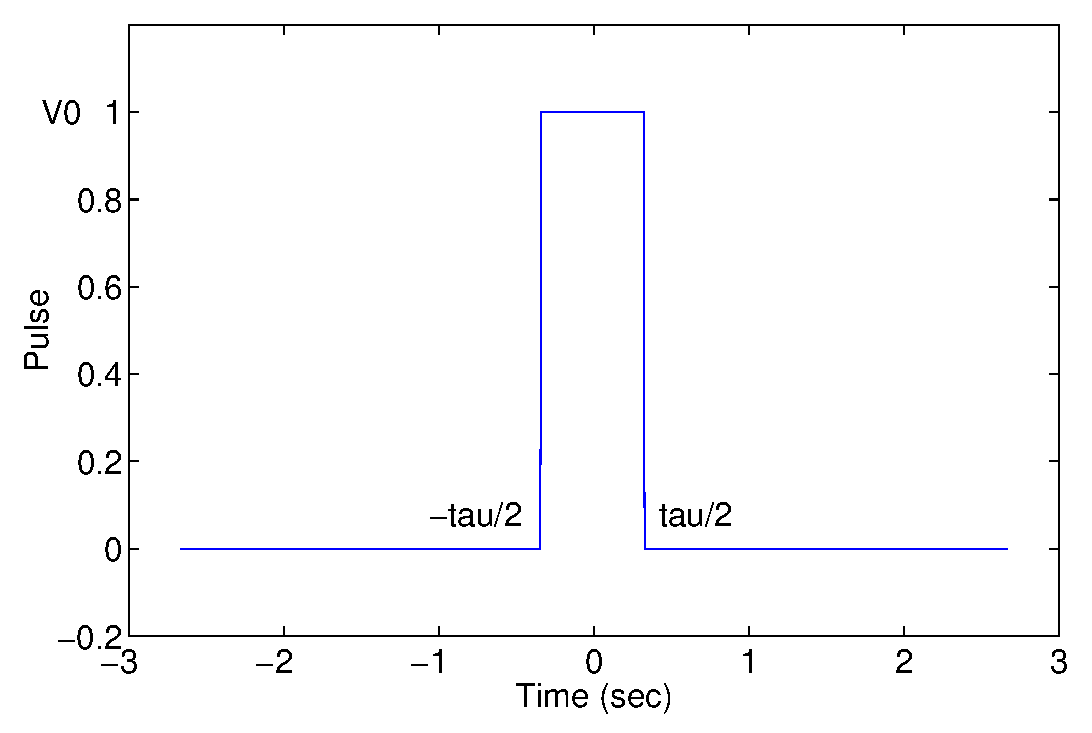
\includegraphics[height=3in]{ch-fft/ft_pulse}}
\caption{A rectangular pulse with width $\tau$. 
\label{fig:ft-pulse-x}}
\end{figure}

Let's look at the rectangular pulse written about before; but here
the pulse is aperiodic --- there is just a single pulse instead of a
train of them. The signal is defined as
\begin{equation}
x(t) = \left\{\begin{array}{ll}
                        1 & |t|\leq \tau/2 \\
                        0   & |t| > \tau/2
                        \end{array}\right.
\end{equation}
and illustrated in Figure~\ref{fig:ft-pulse-x}.  

\begin{figure}
\centerline{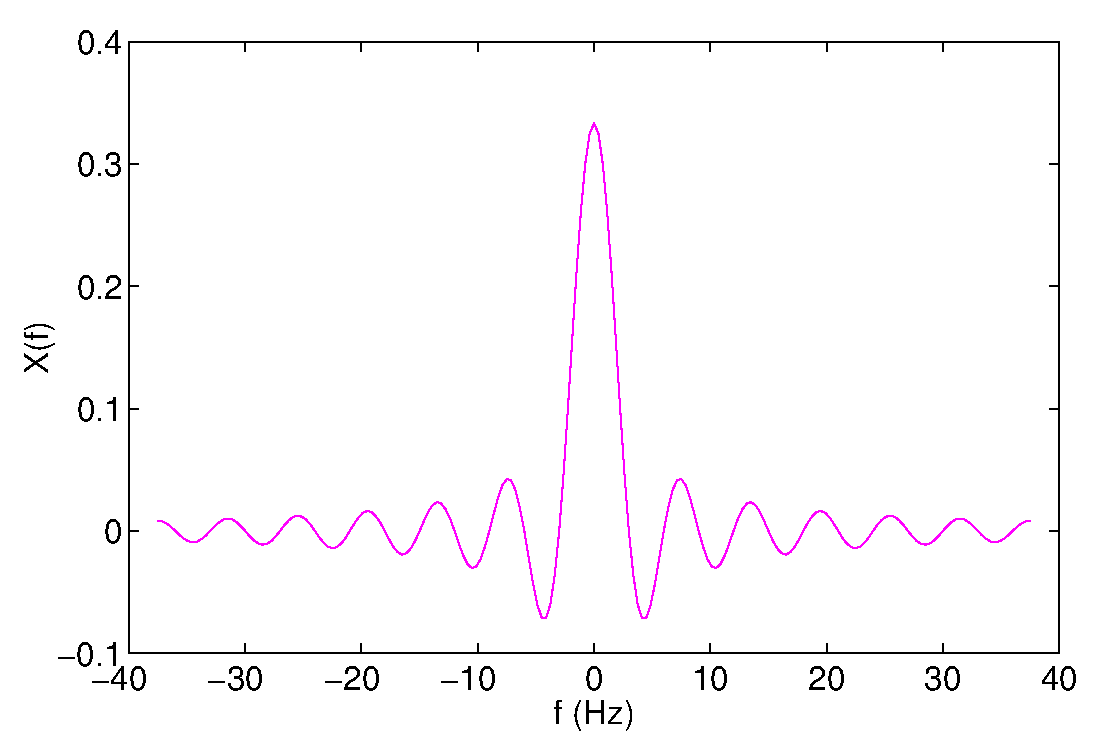
\includegraphics[height=3in]{ch-fft/ft_pulseX}}
\caption{Fourier transform of the pulse in
figure~\protect\ref{fig:ft-pulse-x}.
\label{fig:ft-pulse-X}}
\end{figure}

\index{Fourier Transform!of a pulse}
By applying~(\ref{eq:ft-X}), we find that
\begin{align}
X(f) &= \int_{-\tau/2}^{+\tau/2} e^{-j2\pi ft}dt \notag\\ 
     &= \left.\frac{e^{-j2\pi ft}}
                      {-j2\pi f}\right|_{-\tau/2}^{+\tau/2} \notag\\ 
     &= \frac{1}{-j2\pi f}[e^{-j\pi f\tau}-e^{j\pi f\tau}] \notag\\
     &= \tau\sinc(\pi f \tau)
\label{eq:ft-pulse-X}
\end{align}
The final step in deriving~(\ref{eq:ft-pulse-X}) made use of the
observation that the difference of a complex number and its conjugate
is just twice its imaginary part, $(a-jb) - (a+jb) = -2jb$. In polar
notation, then, $e^{-j\pi f \tau} - e^{j\pi f \tau} = -2j\sin\pi f
\tau$, using Euler's formula. We observe that $X(f)$ is real and has
the shape of the sinc function we mentioned previously. The important
difference here is that it is a \emph{continuous} spectrum instead of
line spectrum.  It is shown in figure~\ref{fig:ft-pulse-X}.

\begin{figure}
\centerline{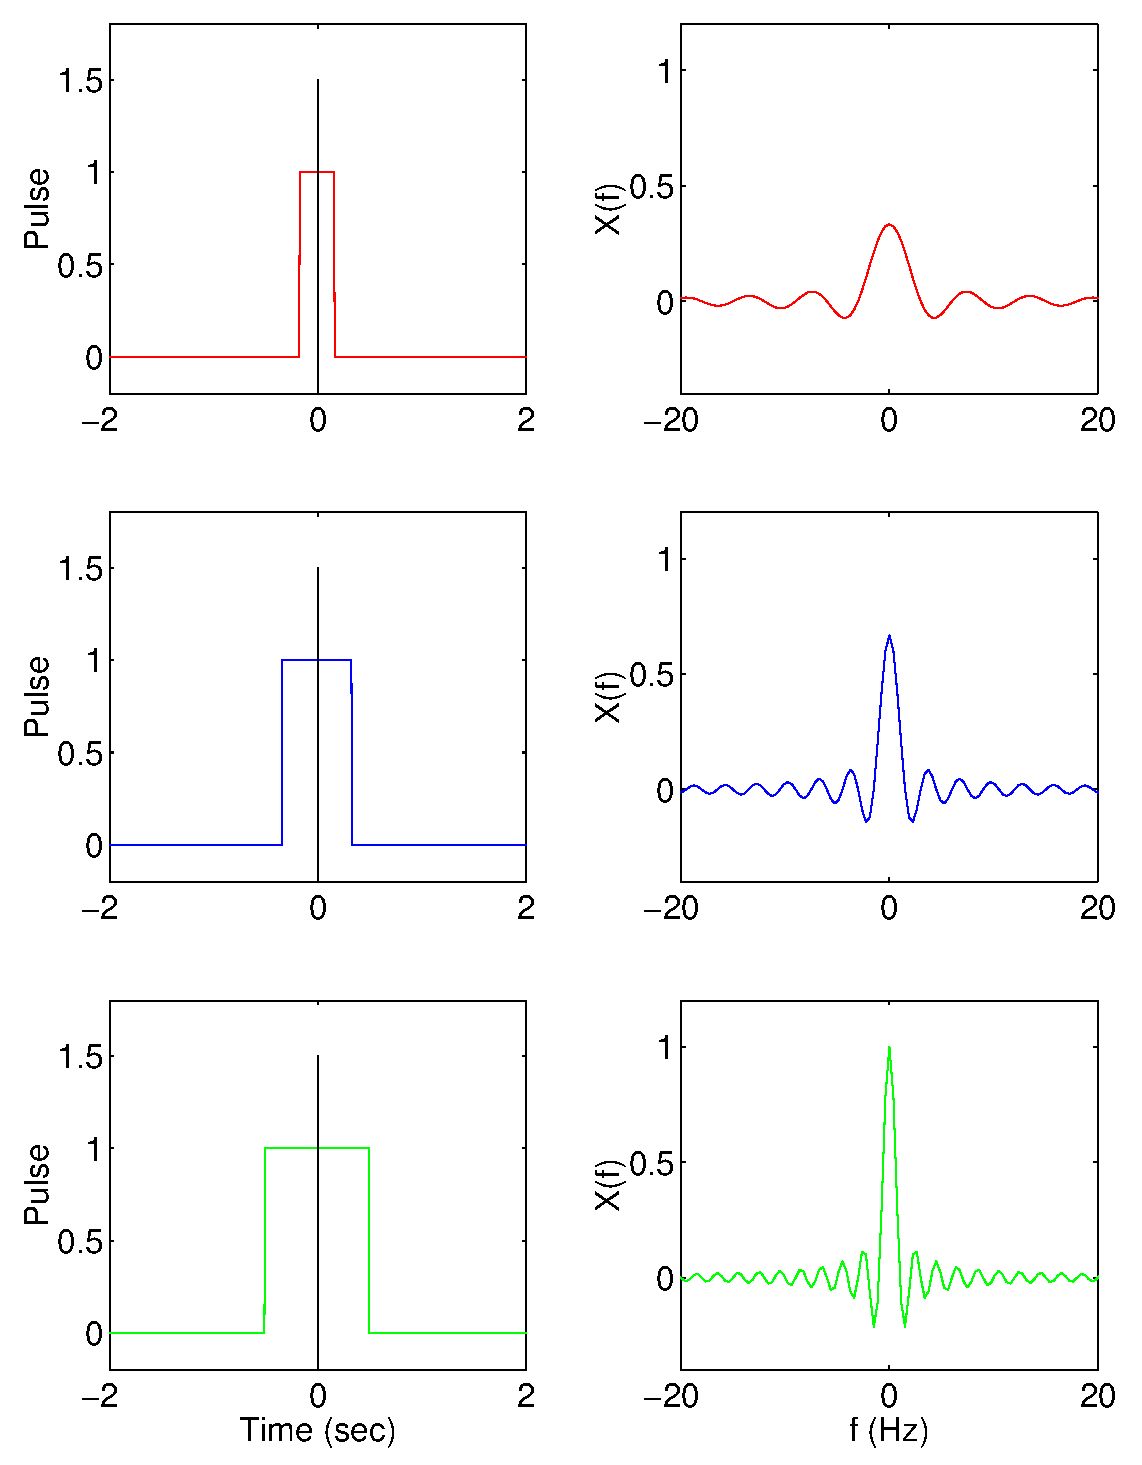
\includegraphics[width=5in]{ch-fft/ft_pulse_xX}}
\caption[Fourier transform of a rectangular pulse for various width 
values]{Fourier transform of a rectangular pulse for various width
values $\tau$.\label{fig:ft-pulse-xX}}
\end{figure}

As with the periodic rectangular pulses, from~(\ref{eq:ft-pulse-X}) we
note that the zero crossings of $X(f)$ occur at multiples of $1/\tau$.
Furthermore, the width of the main lobe, which contains most of the
signal energy, is equal to $1/\tau$. As the pulse duration $\tau$
decreases or increases, the main lobe becomes broader or narrower, and
more energy is moved to the higher or lower frequencies, respectively,
as is illustrated in figure~\ref{fig:ft-pulse-xX}. Thus, as the single
pulse is expanded (compressed) in time, its transform is compressed
(expanded) in frequency.

\section{The Discrete Fourier Transform}

So far, we have examined the Fourier series (which is for a
periodic, continuous signal) and its discrete spectrum and the Fourier
transform (which is for an aperiodic, continuous signal) and its
continuous spectrum. Now, we will investigate periodic, \emph{discrete}
signals and their spectra, which are discrete.

Let's consider a finite digital signal $\{x[n]\}$ ($n=0,1,2,\ldots,
N-1$). The discrete Fourier transform (\emph{DFT}) is defined as
\index{Discrete Fourier Transform (DFT)}
\begin{equation}
X[k] = \sum_{n=0}^{N-1} x[n] e^{-j n k 2\pi/N}, \quad k = 0,1,2,\ldots,
N-1
\label{eq:dft}
\end{equation}
where $X$ is the spectrum of $x$, and its synthesis equation or
inverse DFT (\emph{IDFT}) is
\begin{equation}
x[n]=\frac{1}{N} \sum_{k=0}^{N-1} X[k] e^{j n k 2\pi/N}, \quad
n=0,1,2,\ldots, N-1
\label{eq:idft}
\end{equation}

The DFT converts a finite (periodic), discrete signal in
the time domain ($x[n]$) into a finite, discrete spectrum in the frequency
domain ($X[k]$).

We can derive the DFT informally from the Fourier series of a periodic
signal. Let's compare equation~(\ref{eq:dft}) and that for the
coefficients of the Fourier series, equation~(\ref{eq:fs-ck}), which I
repeat here:
\begin{equation}
c_k=\langle f(t), e^{jk\omega_0 t}\rangle = \frac{1}{T}\int_0^T f(t)e^{-jk\omega_0
t}dt
\label{eq:fs-ckrepeat}
\end{equation}

First, notice that the DFT uses a summation within $[0, N-1]$ and the
series uses an integral within one period T.  This difference arises
because here the signal is discrete and finite (and so we write $x[n]$
instead of $f(t)$). The factor of $1/T$ in~(\ref{eq:fs-ckrepeat}) is
equivalent to that of $1/N$ in~(\ref{eq:idft}), where 
that factor has been arbitrarily included in the IDFT instead of the DFT.

Now let's compare the basis (the complex exponential). The frequency
here is also discretized.  Remember that a sampled signal has a
Nyquist frequency of $\omega_s/2$, or $\pi$ radians/sample, where
$\omega_s$ is the sampling rate, equivalent to $2\pi$ radians/sample.
Let's discretize this signal's frequencies using $N$ equally-spaced
points.  The step $\Delta\hat{\omega}$ between neighboring frequencies (in
radians/sample) is
\begin{equation}
\Delta\hat{\omega} = \frac{2\pi}{N}
\end{equation}
This is what equation~(\ref{eq:dft}) indicates within the sum: that
whatever $nk$ is, it will be a multiple of $2\pi/N$.  The
$k^\mathrm{th}$ frequency in radians can be written as
\begin{equation}
k \Delta\hat{\omega} = k\frac{2\pi}{N}, \quad k = 0, 1, 2, \ldots, N-1
\label{eq:dft-w}
\end{equation}

Substituting $k \Delta\hat{\omega}$ in~(\ref{eq:dft-w}) for
$k\omega_0$ in the Fourier series basis should convince you that the
DFT is the discrete version of the Fourier series. The coefficient
$X[k]$ is the magnitude of the spectrum of $x$ at frequency $k2\pi/N$.

\begin{table}
  \centering
  \begin{tabular}{|l|l|l|l|l|l|} \hline
    $T$ (s) & $f_s$ (Hz) & $N$ & $\Delta\hat{\omega}$ (rad/sample) &
    $\Delta\omega$ (rad/s) & $\Delta f$ (Hz) \\ \hline
    1    & 10    & 10    & $\pi/5$    & $2\pi$    & 1 \\
    10   & 10    & 100   & $\pi/50$   & $\pi/5$   & $1/10$ \\
    100  & 10    & 1000  & $\pi/500$  & $\pi/50$  & $1/100$ \\
    100  & 5     & 500   & $\pi/250$  & $\pi/50$  & $1/100$ \\
    100  & 1     & 100   & $\pi/50$   & $\pi/50$  & $1/100$ \\ \hline
  \end{tabular}
  \caption{Some examples of how $\Delta\hat{\omega}$,
    $\Delta\omega=\Delta\hat{\omega}f_s$, 
    and $\Delta f=\Delta\omega/2\pi = f_s/N$ change for signals of
    different duration and sampling rate.} 
  \label{tb:delta-f}
\end{table}

Table~\ref{tb:delta-f} illustrates how the step between frequencies
changes as the signal duration and sampling rate (and thus number of
samples) change. Increasing the signal duration, and therefore the
number of samples, without changing the sampling rate (which keeps the
Nyquist cutoff constant) decreases the step between frequencies (or,
if you prefer to think of this another way, increases the frequency
resolution). On the other hand, decreasing the sampling rate decreases
the number of samples (assuming the signal duration stays constant)
and the Nyquist cutoff, so the step between frequencies stays
constant.

\subsection{Derivation of the IDFT [\textsc{Optional}]}

Next, let's see how we can get the synthesis equation IDFT from the
DFT. Multiplying both sides of~(\ref{eq:dft}) by $e^{j n' k 2\pi/N}$
and then summing over all $k$,
\begin{equation}
\sum_{k=0}^{N-1} X[k] e^{j n' k 2\pi/N} 
= \sum_{k=0}^{N-1}\sum_{n=0}^{N-1} x[n] e^{-j n k 2\pi/N}e^{j n' k
2\pi/N} 
\end{equation}
Switching the order of summation of $n$ and $k$ on the right side,
plus some algebraic rearrangement yields
\begin{equation}
\sum_{k=0}^{N-1} X[k] e^{j n' k 2\pi/N}
= \sum_{n=0}^{N-1} x[n] \sum_{k=0}^{N-1} e^{j k(n'-n)
2\pi/N}
\label{eq:dft-2idft1}
\end{equation}
It can be shown that
\begin{align}
\sum_{k=0}^{N-1} e^{j k(n'-n)2\pi/N} 
&= \left\{\begin{array}{ll}
                        N & n=n' \\
                        0 & n \neq n'
           \end{array}\right.\\
&= N\delta[n-n']
\end{align}
where $\delta[n-n']$ is defined as
\begin{equation}
\delta[n-n'] = \left\{\begin{array}{ll}
                        1 & n=n' \\
                        0 & n \neq n'
                      \end{array}\right.
\end{equation}

Substituting the above result into~(\ref{eq:dft-2idft1}), we get the
IDFT (but for that pesky factor of $1/N$):
\begin{align}
\sum_{k=0}^{N-1}X[k] e^{j n' k 2\pi/N}
  &= \sum_{n=0}^{N-1}x[n] N\delta[n-n'] \notag\\
  &= Nx[n']
\end{align}

To simplify the notation, let's use a vector notation for the
discrete signal $\mathbf{x}=\{x[n]\}$ and its spectrum
$\mathbf{X}=\{X[k]\}$.  The DFT and IDFT operations become $N\times N$
matrices $\mathbf{F}$ and $\mathbf{F^{-1}}$, respectively. An element
in row $k$ and column $n$ of $\mathbf{F}$ is
\begin{equation}
[\mathbf{F}]_{kn}= e^{-jnk2\pi/N}, \quad k,n=0,1,2,\ldots,N-1
\end{equation}
Then the DFT and IDFT can be written as
\begin{align}
\mathbf{X} &= \mathbf{F}\mathbf{x}\\
\mathbf{x} &= \mathbf{F^{-1}}\mathbf{X}
\end{align}
or 
\begin{gather}
\mathbf{x}\stackrel{\mathbf{F}}{\longrightarrow} \mathbf{X}\\
\mathbf{X}\stackrel{\mathbf{F^{-1}}}{\longrightarrow} \mathbf{x}
\end{gather}

\subsection{Finite vs. Infinite Signals}

In this book, we have used (and will continue to use) the terms
``periodic'' and ``finite'' interchangeably (and, similarly,
``aperiodic'' and ``infinite''). When we compute the Fourier series or
the DFT of a finite signal of duration $T$, we do so only within that
interval of time. In effect, what we are doing for finite signals is
``pretending'' that the signal is actually periodic with period $T$
and that we are only looking at one of its periods.

On the other hand, if a signal is actually of infinite duration, we
would use the Fourier transform. However, this is not a process that
we can perform on a computer, where infinite duration signals cannot
exist (the duration of any signal is limited by the available
storage). We have to chop the signal off at a length that the computer
can handle, ignoring the error it may produce (or testing to make sure
that the error is tolerable for our application). This brings us back
to the DFT for processing the resulting finite signal as an
\emph{approximation} of the infinite signal's Fourier transform. Note
that, even outside the computer, our time is finite (even the lifespan
of the universe is finite) and so no physically realizable signal is
actually infinite.


\subsection{Properties of the DFT}

\index{Discrete Fourier Transform (DFT)!properties of}
Let's consider some of the properties of the DFT of physically
realizable signals. These signals are real, so $x[n] = x[n]^*$. What
is the spectrum of such a signal like? We can think of the signal's
frequency content or spectrum, $X[k]$ ($k=0,1,\ldots,N-1$), as a
sequence of $N$ complex numbers. This is known as a \emph{$N$ point
FFT}. If we compute $X[N-k]$ using~(\ref{eq:dft}), we get
\index{FFT!points}
\begin{align*}
X[N-k] &= \sum_{n=0}^{N-1} x[n] e^{-j n (N-k) 2\pi/N} \\
&= \sum_{n=0}^{N-1} x[n] e^{-jn2\pi}e^{j n k 2\pi/N} \\
&= \sum_{n=0}^{N-1} x[n] e^{j n k 2\pi/N} &&\text{(since $e^{-jn2\pi}=1$)}\\
&= \left[\sum_{n=0}^{N-1} x[n]^* e^{-j n k 2\pi/N}\right]^* 
   &&\text{(since $ab = ((ab)^*)^* = (a^*b^*)^*$)}
\end{align*}
Because $x[n]=x[n]^*$,
\begin{align}
X[N-k]&= \left[\sum_{n=0}^{N-1} x[n] e^{-j n k 2\pi/N}\right]^* \notag\\
       &= X[k]^*
\end{align}

So for example, when $N=8$, $k=0, 1,2,3,4,5,6,7$, and
\begin{equation}
X[7]=X[1]^* \quad X[6]=X[2]^* \quad X[5]=X[3]^*
\end{equation}
(When $k=0$, $X[8]=X[0]^*$ but $X[8]$ is out of spectrum, which ranges
from 0 to 7 only. This is the ``DC'', or zero-frequency, component of
the signal.)

This can be represented diagrammatically as
\begin{equation}
\underset{\underset{\text{DC}}{\uparrow}}{0} \quad \underbrace{1 \quad
    \overbrace{2 \quad \underbrace{3 \quad 4 \quad 5} \quad 6} \quad 7}
\label{eq:dft8-freqs}
\end{equation}
This is clearly symmetric about $k=4$. When $N$ is an even number,
the spectrum has $N/2$ at the center; when $N$ is an odd number, the
center is between $\lfloor N/2 \rfloor$ and $\lceil N/2 \rceil$. So,
for $N=7$,
\begin{equation}
\underset{\underset{\text{DC}}{\uparrow}}{0} \quad \underbrace{1 \quad
  \overbrace{2 \quad \underbrace{3 \quad 4} \quad 5} \quad 6}
\end{equation}   

What this means is that the spectrum over frequencies $\lceil N/2
\rceil$ to $N-1$ has the same magnitude as over 1 to $\lfloor N/2
\rfloor$, but with negative phase angle (which means negative
frequencies on the unit circle). In fact, $N/2$ corresponds to the
Nyquist frequency in radians/sample. We can see this
from~(\ref{eq:dft-w}), when $k=N/2$
\begin{equation}
\hat{\omega}_{N/2}=\frac{N}{2}\frac{2\pi}{N}=\pi
\end{equation}
Converting this to Hz, we get
\begin{equation}
\hat{f}_{N/2} = \hat{\omega}_{N/2}\frac{f_s}{2\pi}
              = \pi\frac{f_s}{2\pi} = \frac{f_s}{2}
\end{equation}
where $f_s$ is the sampling rate. The above equation shows that
$\hat{f}_{N/2}$ is the Nyquist frequency in Hz. The conclusion is that
the magnitude of the transform of a real valued signal is an
\emph{even} function of frequency and so we only need to plot its
spectrum in range $[0, N/2]$, corresponding to the range of
frequencies from 0 to the Nyquist frequency. This also means that the
DFT of a real signal has (slightly more than) half the information of
the DFT of a complex-valued signal with the same number of samples
(which makes sense, since each sample has an imaginary component of
zero).

\problemset{
\subsubsection{Self-Test Exercises}

See~\ref{sc:ch7ex} \#\ref{it:ch5ex4} for the answer.

\begin{enumerate}
\item Show which frequencies will be equal for a spectrum with:
  \begin{enumerate}
  \item 16 points.
  \item 15 points.
  \end{enumerate}
\end{enumerate}}

\subsubsection{Example: Spectrum of an exponential}

\begin{figure}
\centerline{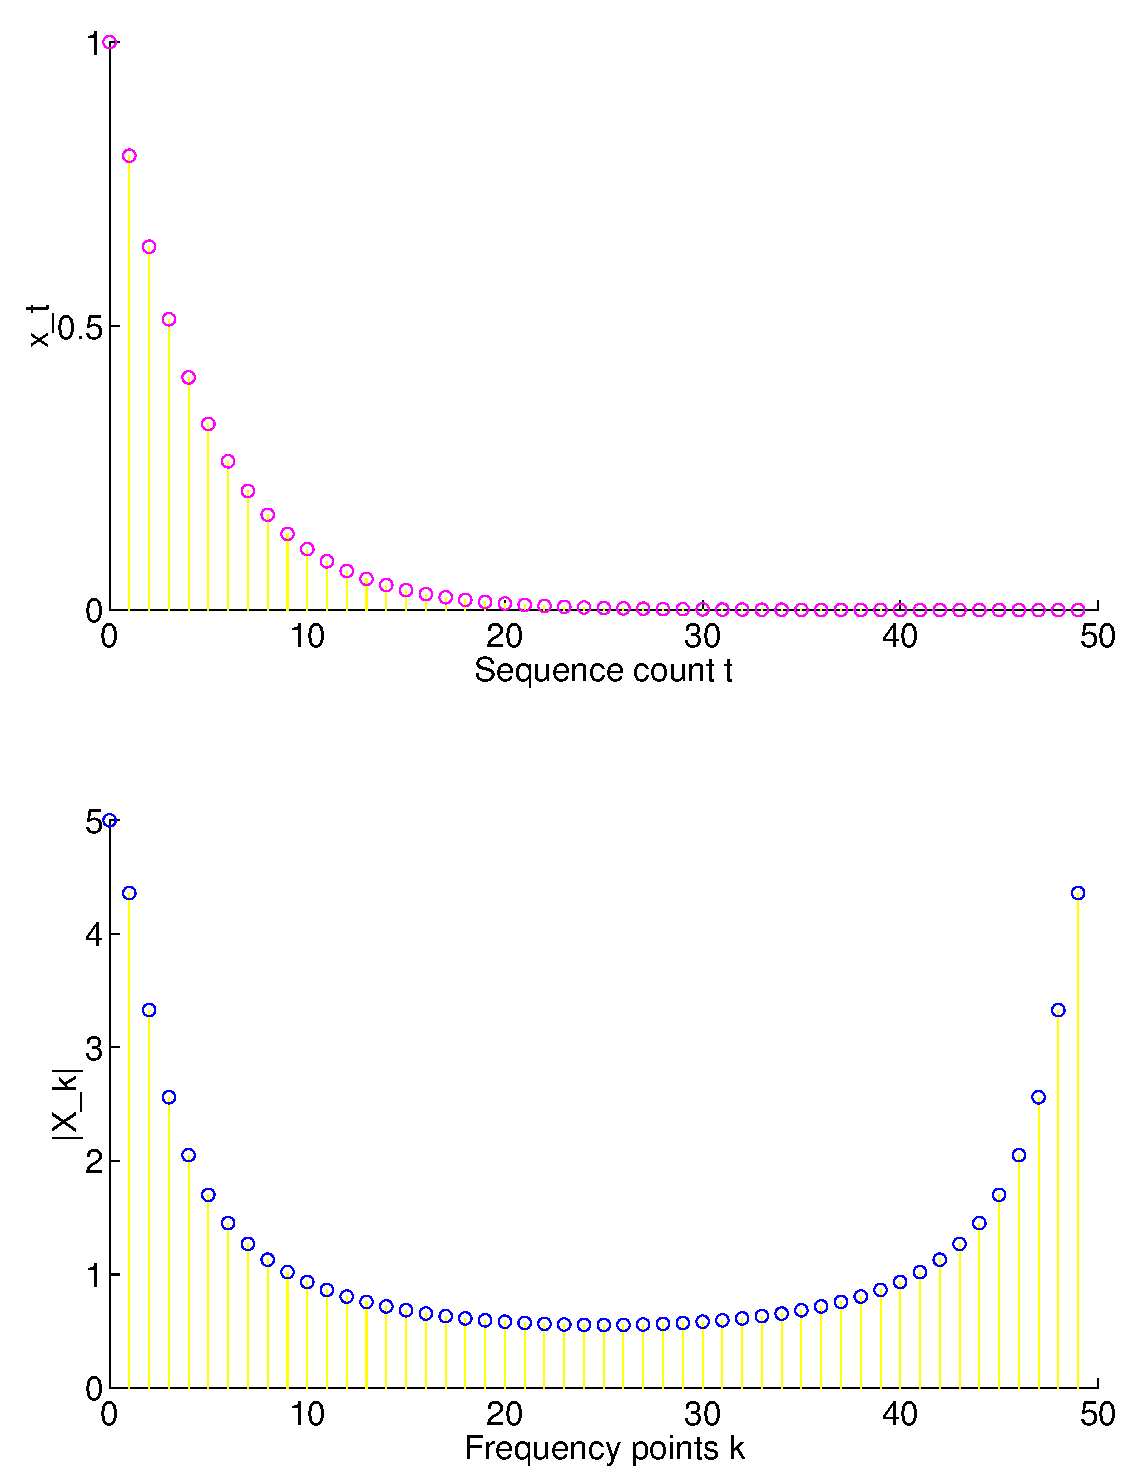
\includegraphics[width=5in]{ch-fft/dft_expxX}}
\caption[Plot of the sequence {$x[n] = 0.8^n$} and the
magnitude of its DFT]{Plot of the sequence $x[n] = a^n$, $0<a<1$ (top)
and the magnitude of its DFT (bottom), where $a=0.8$ and $N=50$.
\label{fig:dft-exp-xX}}
\end{figure}

Consider the exponential signal 
\begin{equation}
x[n] = a^n, \quad 0<a<1, \quad n = 0,1,2,\ldots,N-1
\end{equation}
The signal is plotted in the top of figure~\ref{fig:dft-exp-xX}

The DFT of the sequence $x[n]$ is 
\index{Discrete Fourier Transform (DFT)!of an exponential}
\begin{align}
X[k] &= \sum_{n=0}^{N-1} x[n] e^{-jnk2\pi/N} \notag\\
     &= \sum_{n=0}^{N-1} a^n e^{-jnk2\pi/N}
  \label{eq:exp-dft1}
\end{align}
The common ratio for this geometric series (the ratio of two
\index{geometric series!common ratio}
successive terms) is $ae^{-jk2\pi/N}$.  Accordingly, the summation
in~(\ref{eq:exp-dft1}) becomes
\begin{align}
X[k] &= \frac{1-a^Ne^{-jkN2\pi/N}}{1-ae^{-jk2\pi/N}} \notag\\
     &= \frac{1-a^N}{1-ae^{-jk2\pi/N}}
\end{align}

\begin{figure}
\centerline{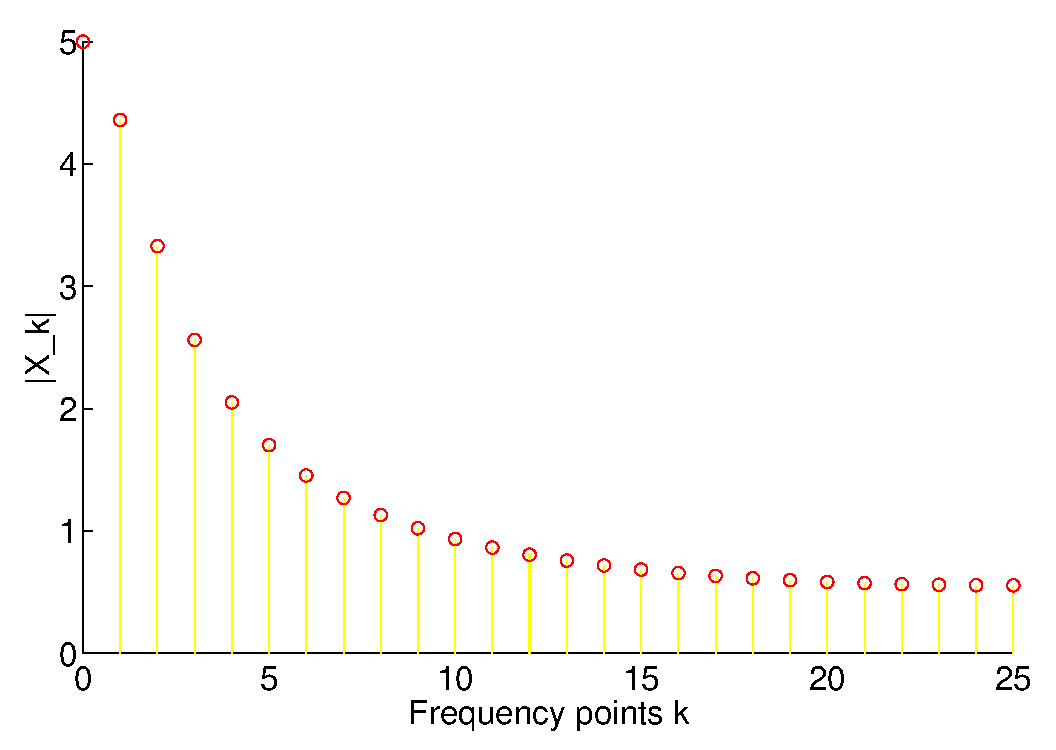
\includegraphics[height=3.5in]{ch-fft/dft_expX2}}
\caption[First half of DFT of {$x[n] = 0.8^n$}]{Magnitude of DFT for the
signal~\protect\ref{fig:dft-exp-xX} top is plotted for the first half
of its range.
\label{fig:dft-exp-X2}}
\end{figure}

The magnitude of $X[k]$ for $N=50$ and $a=0.8$ is plotted in the bottom
of figure~\ref{fig:dft-exp-xX}.  Since this is a real signal, $|X[k]|$
is an even function of frequency, and so we can just plot the first
half of the range of 0 to $N/2$. That is shown in
figure~\ref{fig:dft-exp-X2}

\subsection{Computing the DFT Directly}

\index{Discrete Fourier Transform (DFT)!direct computation}
Later on, a method for computing the DFT efficiently will be introduced.
In view of the importance of the DFT in various digital signal
processing applications, such as linear filtering, correlation
analysis, and spectrum analysis, its efficient computation is a topic
that has received considerable attention by many mathematicians,
engineers, and applied scientists. But, let's first consider the
direct, brute-force approach.

To compute the DFT, we need to compute the sequence $\{X[k]\}$ of $N$
complex-valued numbers given another sequence of data $\{x[n]\}$ of
length $N$, according to the formula~(\ref{eq:dft}):
\begin{equation*}
X[k] = \sum_{n=0}^{N-1} x[n] e^{-j n k 2\pi/N}, \quad k = 0,1,2,\ldots,
N-1
\end{equation*}

\index{Discrete Fourier Transform (DFT)!direct computation!complexity}
In general, the data sequence $x[n]$ is also assumed to be complex
valued. We observe that for each value of $k$, direct computation of
$X[k]$ involves $N$ complex multiplications ($4N$ real multiplications
and $2N$ real additions) and $N-1$ complex additions ($2N-2$ real
additions). Consequently, to compute all $N$ values of the DFT
requires $4N^2$ complex multiplications and $4N^2-2N$ complex
additions. So, the direct approach is an $O(N^2)$ algorithm, and you
should recognize that this is not terribly efficient to say the
least.

\subsection{The Fast Fourier Transform Algorithm}
\label{sc:fft}

\index{Discrete Fourier Transform (DFT)!FFT}
The development of computationally efficient algorithms for the DFT is
made possible if we adopt a divide-and-conquer approach, called Fast
Fourier Transform (\emph{FFT}).  This approach is based on the
decomposition of an $N$ point DFT into successively smaller DFTs, in a
manner similar to how mergesort or quicksort divide large sorting
problems into smaller sorting problems.

A DFT of length $N$ can be rewritten as the sum of two DFTs, each of
length $N/2$. One of the two is formed from the even-numbered points
of the original $N$, while the other uses the odd-numbered
points. This division can be arrived at straightforwardly:
\begin{align}
X[k] &= \sum_{n=0}^{N-1} x[n] e^{-jnk2\pi/N} \notag\\ 
&=
\sum_{n=0}^{N/2-1} x[2n] e^{-jk(2n)2\pi/N}+
\sum_{n=0}^{N/2-1} x[2n+1] e^{-jk(2n+1)2\pi/N}
\notag\\
&=
\sum_{n=0}^{N/2-1} x[2n] e^{-jkn2\pi/(N/2)}+
e^{-jk2\pi/N}\sum_{n=0}^{N/2-1} x[2n+1] e^{-jkn2\pi/(N/2)}
\notag\\
&= X[k]^{\textit{even}} + e^{-jk2\pi/N} X[k]^{\textit{odd}},
    \quad k=0,1,2,\ldots, N-1
\label{eq:fft-xexo}
\end{align}
where 
\begin{align}
X[k]^{\mathit{even}} &= \sum_{n=0}^{N/2-1} x[2n] e^{-jkn2\pi/(N/2)} \\
X[k]^{\mathit{odd}}  &= \sum_{n=0}^{N/2-1}x[2n+1] e^{-jkn2\pi/(N/2)}
\end{align}
where $k=0, 1, 2, \ldots, N/2-1$.

$X[k]^{\mathit{even}}$ denotes the $k^{\textrm{th}}$ component of the
DFT of length $N/2$ formed from the even components of the original
$x[n]$, while $X[k]^{\mathrm{odd}}$ is the corresponding transform of
length $N/2$ formed from the odd components. The transforms
$X[k]^{\mathit{even}}$ and $X[k]^{\mathit{odd}}$ are periodic in $k$
with length $N/2$. So each is repeated through two cycles to obtain
$X[k]$:
\begin{align}
X[k+N/2]^{\mathit{even}} &= \sum_{n=0}^{N/2-1} x[2n] e^{-j(k+N/2)n2\pi/(N/2)}
\notag\\
&= \sum_{n=0}^{N/2-1} x[2n] e^{-jkn2\pi/(N/2)}=X[k]^{\mathit{even}} 
\label{eq:fft-repeat-even}
\\
X[k+N/2]^{\mathit{odd}} &= \sum_{n=0}^{N/2-1} x[2n+1] e^{-j(k+N/2)n2\pi/(N/2)}
\notag\\
&= \sum_{n=0}^{N/2-1} x[2n+1] e^{-jkn2\pi/(N/2)}=X[k]^{\mathit{odd}}
\label{eq:fft-repeat-odd}
\end{align}
because $e^{-jkn2\pi}=1$. 

The good thing is that this process can be continued recursively, just
as in the divide-and-conquer sorting algorithms. Having reduced the
problem of computing $X[k]$ to that of computing
$X[k]^{\mathit{even}}$ and $X[k]^{\mathit{odd}}$, we can do the same
reduction of $X[k]^{\mathit{even}}$ to the problem of computing the
transform of its $N/4$ even-numbered elements and $N/4$ odd-numbered
elements. In other words, we can define $X[k]^{\mathit{even-even}}$
and $X[k]^{\mathit{even-odd}}$ to be DFT of the points which are
respectively even-even and even-odd on the successive subdivisions of
the data. The same process can be applied to recursively divide
$X[k]^{\mathit{odd}}$.

It is easy to imagine continuing this process until the DFT size is
one, if $N$ is a power of two. Though there are special algorithms if
$N$ is not a power of two, we can assume that the data is just padded
with zeros up to the next power of two. Having done that, we will
continue developing the FFT algorithm for $N$ a power of two as a
general-purpose DFT algorithm. With this condition on $N$, we can
continue applying the dividing method until we have subdivided the
data all they way down to transforms of length 1. The DFT of $x[n]$ for
some $n$, and $N=1$ is $x[n]$! Therefore,
\begin{equation}
X[k]^\mathit{even-even-odd-\cdots} = x[n], \quad \text{for some } n
\end{equation}

The results of adjacent pairs of these one-point DFTs can be merged
using~(\ref{eq:fft-xexo}): $X[k]^{\mathit{even}} +
e^{-jk2\pi/N}X[k]^{\mathit{odd}}$. In this case $k=\{0,1\}$, $N=2$,
and the one-point DFTs are the even and odd signal values themselves,
so this reduces to,
\begin{align}
  X_2[0] &= x[\mathit{even}] + e^{-j(0)2\pi/2}x[\mathit{odd}] \notag \\
         &= x[\mathit{even}] + x[\mathit{odd}] \label{eq:2fft-even}\\
  X_2[1] &= x[\mathit{even}] + e^{-j(1)2\pi/2}x[\mathit{odd}] \notag \\
         &= x[\mathit{even}] - x[\mathit{odd}] \label{eq:2fft-odd}
\end{align}
where the subscript ``2'' has been used to indicate that this is a
2-point DFT.

\begin{algorithm}
\caption{Recursive FFT.\label{alg:fft-recursive}}
\begin{algorithmic}
\REQUIRE $x$ is a discrete function of time of length $N=2^m$
\ENSURE $X$ is the DFT of $x$ (also of length $N$)
\IF{$N = 1$}
   \STATE Return $x$
\ELSE
   \STATE Divide $x$ into $x^\mathit{even}$ and $x^\mathit{odd}$
          \COMMENT{the even and odd numbered points}
   \STATE $X^\mathit{even} = \operatorname{FFT}(x^\mathit{even})$
   \STATE $X^\mathit{odd} = \operatorname{FFT}(x^\mathit{odd})$
   \FOR{$k=0, 1, 2, \ldots, N-1$}
      \STATE $X_N[k] = X_{N/2}[k]^\mathit{even} +
                       e^{-jk2\pi/N}X_{N/2}[k]^\mathit{odd}$ 
   \ENDFOR
   \STATE Return $X$
\ENDIF
\end{algorithmic}
\end{algorithm}

This is the basic FFT.  High-level pseudocode for a recursive
implementation is given in algorithm~\ref{alg:fft-recursive}, where I
have used subscripts to distinguish between the values of the
$N/2$-point FFT and the $N$-point FFT. The base case for the recursion
is that the length of the signal is one. As I'm sure you're familiar,
recursive algorithms are short, simple, and elegant, but not always as
efficient as non-recursive ones.  There is a non-recursive approach to
the even and odd dividing, and it is really neat, so I'll go over it.

\begin{table}
\caption{Example of the effect of bit reversal on an eight-element
input vector.\label{tb:fft-bitrevers}}
\begin{center}
\begin{tabular}{|c|c|c|c|} \hline
 \multicolumn{2}{|c|}{Input} & 
\multicolumn{2}{c|}{Bit-Reversed Result} \\ \hline
Decimal & Binary & Binary & Decimal \\ \hline\hline
0 & 000 & 000 & 0\\
1 & 001 & 100 & 4\\
2 & 010 & 010 & 2\\
3 & 011 & 110 & 6\\
4 & 100 & 001 & 1\\
5 & 101 & 101 & 5\\
6 & 110 & 011 & 3\\
7 & 111 & 111 & 7 \\ \hline
\end{tabular}
\end{center}
\end{table}

We start with the problem of how to sort even and odd numbers and how
to know which $n$ goes to which pattern of
$X[k]^\mathit{even-\cdots}$ and $X[k]^\mathit{odd-\cdots}$. The
successive subdivisions of the data into even and odd parts are tests
of successive low-order (least significant) bits of the binary
representation of $n$. This is true because the least significant bit
of an binary number is what determines if it is even or odd, and the
act of dividing a binary number by two is equivalent to shifting it to
the right one bit, which makes the next bit the new least significant
bit.  We take the original vector of data $x[n]$ and rearrange it into
bit-reversed order (see table~\ref{tb:fft-bitrevers} for an example
for $N=8$), so that the individual numbers are not in order of $n$,
but of the number obtained by bit-reversing $n$. The function of
bit-reversing is to take care of all those even and odd divisions to
the final list for $N$ one-point transforms!

How do we recombine these non-recursively to produce the result?
Starting with the one-point transforms, we combine adjacent pairs to
get two-point transforms according to~(\ref{eq:fft-xexo}), then
combine adjacent pairs of pairs of 4-point transforms, and so on,
until we combine $N/2$ point transforms into the final transform of
$N$ total data points.

\begin{algorithm}
\caption{Iterative FFT.\label{alg:fft}}
\begin{algorithmic}
\REQUIRE $x$ is a discrete function of time of length $N$
\ENSURE $X$ is the DFT of $x$ (also of length $N$)
\IF{$N$ is not a power of two}
   \STATE Pad $x$ with zeros until its length is the next power of two
\ENDIF
\STATE Shuffle the $x[n]$ in bit-reversed order
\STATE $\mathit{Size} = 2$ \COMMENT{$\mathit{Size}=1$ DFTs already done}
\WHILE{$\mathit{Size} \leq N$}
   \STATE Compute $N/\mathit{Size}$ DFTs from the existing ones as
          $X_{\mathit{Size}/2}[k]^{\mathit{even}} +
          e^{-jk2\pi/\mathit{Size}}X_{\mathit{Size}/2}[k]^{\mathit{odd}}$
   \STATE $\mathit{Size} = \mathit{Size} \times 2$
\ENDWHILE
\end{algorithmic}
\end{algorithm}

\begin{figure}
\centerline{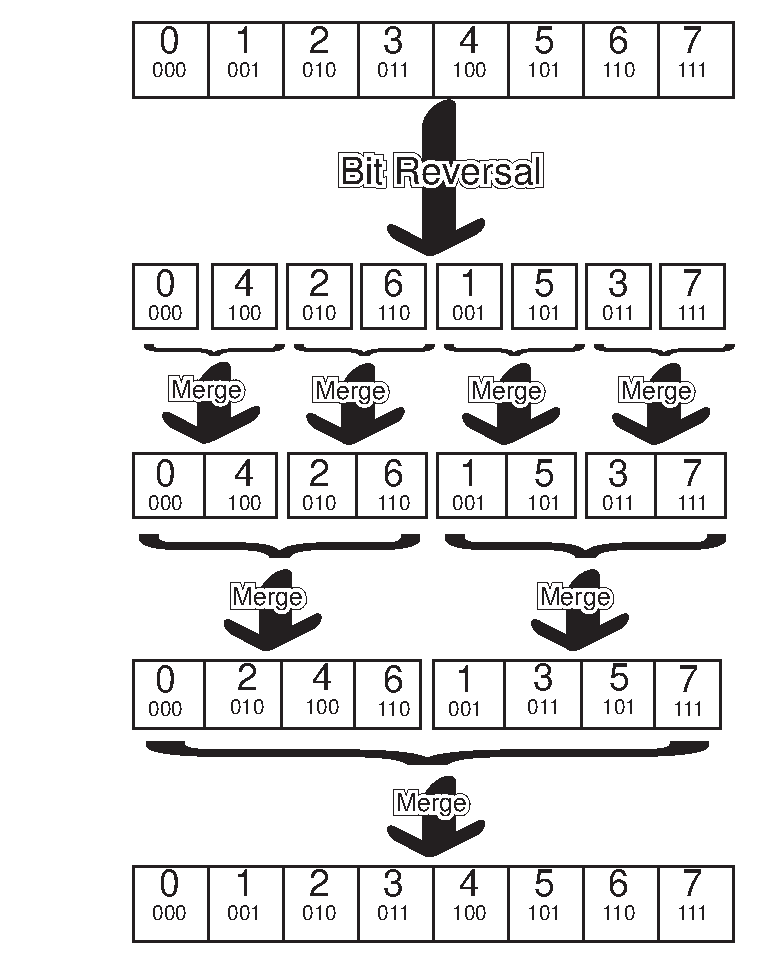
\includegraphics[height=4in]{ch-fft/fft-iterative}}
\caption{Schematic outline of an iterative 8-point FFT
\label{fg:fft-iterative}}
\end{figure}

In summary, the bit-reverse-based nonrecursive FFT algorithm is given
in algorithm~\ref{alg:fft}. This is illustrated in
figure~\ref{fg:fft-iterative}.

As far as the computational complexity of this algorithm is concerned,
each iteration of the loop is $O(N)$ (we're computing
$N/\mathit{Size}$ DFTs, each with $\mathit{Size}$ elements), and the
loop executes $\log_2N$ times, so the whole algorithm is
$O(N\log_2N)$.  Directly computing the DFT (i.e., not using the FFT
algorithm) takes $O(N^2)$.

\subsubsection{Example: 8-Point FFT}

Let's compute the FFT of the signal, $x[n] = \{0, 1, 0, 1, 0, 1, 0,
1\}$, $n = \{0, 1, 2, 3, 4, 5, 6, 7\}$. The first thing we'll do is
write the signal out as a 1D array, with indices in binary:
\begin{center}
  \begin{tabular}{r|c|c|c|c|c|c|c|c|} \hline
    $x[n]$ & 0   & 1   & 0   & 1   & 0   & 1   & 0   & 1   \\ \hline
    $n$ & 000 & 001 & 010 & 011 & 100 & 101 & 110 & 111 \\ \hline
  \end{tabular}
\end{center}

Next, we sort the elements according to their bit-reversed indices:
\begin{center}
  \begin{tabular}{r|c|c|c|c|c|c|c|c|} \hline
    $x[n]$ & 0   & 0   & 0   & 0   & 1   & 1   & 1   & 1   \\ \hline
    $n$ 000 & 100 & 010 & 110 & 001 & 101 & 011 & 111 \\ \hline
  \end{tabular}
\end{center}

Each of these elements is already a 1-point FFT; we now begin merging
them into 2-point ones ($X_2[0]= x[\mathit{even}] + x[\mathit{odd}]$
and $X_2[1]= x[\mathit{even}] - x[\mathit{odd}]$), as in
equations~(\ref{eq:2fft-even}) and~(\ref{eq:2fft-odd}):
\begin{center}
  \begin{tabular}{r|c|c||c|c||c|c||c|c|} \hline
    $X_2[k]$ & 0   & 0   & 0   & 0   & 2   & 0   & 2   & 0   \\ \hline
    $k$        & 0   & 1   & 0   & 1   & 0   & 1   & 0   & 1   \\ \hline
  \end{tabular}
\end{center}

Now we have four 2-point FFTs; we now merge adjacent pairs of
points. So, we will be computing $X_4[k]$ for $k=\{0, 1, 2, 3\}$. To
compute elements $k=2$ and $k=3$, we need to remember
equations~(\ref{eq:fft-repeat-even}) and~(\ref{eq:fft-repeat-odd}) ---
that, since the transform $X$ is periodic, we simply repeat the
2-point FFTs to get the ``extra'' two points. So, $X_2[2] = X_2[0]$
and $X_2[3] = X_2[1]$. The resulting equations are:
\begin{align*}
  X_4[0] &= X_2[0]^{\mathit{even}} +   e^{-j(0)2\pi/4}X_2[0]^{\mathit{odd}} \\
  X_4[1] &= X_2[1]^{\mathit{even}} +   e^{-j(1)2\pi/4}X_2[1]^{\mathit{odd}} \\
  X_4[2] &= X_2[0]^{\mathit{even}} +   e^{-j(2)2\pi/4}X_2[0]^{\mathit{odd}} \\
  X_4[3] &= X_2[1]^{\mathit{even}} +   e^{-j(3)2\pi/4}X_2[1]^{\mathit{odd}}
\end{align*}

We can do the arithmetic in the exponents,
\begin{align*}
  X_4[0] &= X_2[0]^{\mathit{even}} +   e^0 X_2[0]^{\mathit{odd}} \\
  X_4[1] &= X_2[1]^{\mathit{even}} +   e^{-j\pi/2} X_2[1]^{\mathit{odd}} \\
  X_4[2] &= X_2[0]^{\mathit{even}} +   e^{-j\pi} X_2[0]^{\mathit{odd}} \\
  X_4[3] &= X_2[1]^{\mathit{even}} +   e^{-j3\pi/2}X_2[1]^{\mathit{odd}}
\end{align*}
and then simplify,
\begin{align*}
  X_4[0] &= X_2[0]^{\mathit{even}} +   X_2[0]^{\mathit{odd}} \\
  X_4[1] &= X_2[1]^{\mathit{even}} -   j X_2[1]^{\mathit{odd}} \\
  X_4[2] &= X_2[0]^{\mathit{even}} -   X_2[0]^{\mathit{odd}} \\
  X_4[3] &= X_2[1]^{\mathit{even}} +   j X_2[1]^{\mathit{odd}}
\end{align*}
yielding:
\begin{center}
  \begin{tabular}{r|c|c|c|c||c|c|c|c|} \hline
    $X_4[k]$ & 0   & 0   & 0   & 0   & 4   & 0   & 0   & 0   \\ \hline
    $k$        & 0   & 1   & 2   & 3   & 0   & 1   & 2   & 3   \\ \hline
  \end{tabular}
\end{center}

We repeat this process one more time to get the 8-point final result,
\begin{align*}
  X_8[0] &= X_4[0]^{\mathit{even}} +  e^{-j(0)2\pi/8}X_4[0]^{\mathit{odd}} \\
  X_8[1] &= X_4[1]^{\mathit{even}} +  e^{-j(1)2\pi/8}X_4[1]^{\mathit{odd}} \\
  X_8[2] &= X_4[2]^{\mathit{even}} +  e^{-j(2)2\pi/8}X_4[2]^{\mathit{odd}} \\
  X_8[3] &= X_4[3]^{\mathit{even}} +  e^{-j(3)2\pi/8}X_4[3]^{\mathit{odd}} \\
  X_8[4] &= X_4[0]^{\mathit{even}} +  e^{-j(4)2\pi/8}X_4[0]^{\mathit{odd}} \\
  X_8[5] &= X_4[1]^{\mathit{even}} +  e^{-j(5)2\pi/8}X_4[1]^{\mathit{odd}} \\
  X_8[6] &= X_4[2]^{\mathit{even}} +  e^{-j(6)2\pi/8}X_4[2]^{\mathit{odd}} \\
  X_8[7] &= X_4[3]^{\mathit{even}} +  e^{-j(7)2\pi/8}X_4[3]^{\mathit{odd}}
\end{align*}
producing:
\begin{align*}
  X_8[0] &= X_4[0]^{\mathit{even}} +  X_4[0]^{\mathit{odd}} \\
  X_8[1] &= X_4[1]^{\mathit{even}} +  e^{-j\pi/4}X_4[1]^{\mathit{odd}} \\
  X_8[2] &= X_4[2]^{\mathit{even}} -  j X_4[2]^{\mathit{odd}} \\
  X_8[3] &= X_4[3]^{\mathit{even}} +  e^{-j3\pi/4}X_4[3]^{\mathit{odd}} \\
  X_8[4] &= X_4[0]^{\mathit{even}} -  X_4[0]^{\mathit{odd}} \\
  X_8[5] &= X_4[1]^{\mathit{even}} +  e^{-j5\pi/4}X_4[1]^{\mathit{odd}} \\
  X_8[6] &= X_4[2]^{\mathit{even}} +  jX_4[2]^{\mathit{odd}} \\
  X_8[7] &= X_4[3]^{\mathit{even}} +  e^{-j7\pi/4}X_4[3]^{\mathit{odd}}
\end{align*}

The final result is:
\begin{center}
  \begin{tabular}{r|c|c|c|c|c|c|c|c|} \hline
    $X_8[k]$ & 4   & 0   & 0   & 0   & -4  & 0   & 0   & 0   \\ \hline
    $k$        & 0   & 1   & 2   & 3   & 4   & 5   & 6   & 7   \\ \hline
  \end{tabular}
\end{center}

To interpret this, since we're dealing with a real-valued signal, we
refer back to~(\ref{eq:dft8-freqs}). $X_8[0]$ is the DC value,
proportional to the mean value of the signal (in fact, it would be
equal to the mean if we divide by $N$). We need only examine elements
1 through 4, since the spectrum is periodic. Only element 4 is
nonzero. This makes sense, since the original signal repeated every
other sample, which is right at the Nyquist frequency ($\pi$),
corresponding to element 4.

\problemset{
\subsubsection{Self-Test Exercises}

See~\ref{sc:ch7ex} \#\ref{it:ch5ex5}--\ref{it:ch5ex6.5} for answers.

\begin{enumerate}
\item Prove that the DFT of $x[n]$ for any $n=m$ and $N=1$ is $x[m]$.
\item Perform step-by-step division for the example given in
  table~\ref{tb:fft-bitrevers} to prove the final result is equal to the
  bit-reversed input.
\item Perform the 4-point FFT of the signal $x[n] = \{1, 2, 3, 4\}$,
  $n = \{0, 1, 2, 3\}$ by hand.
\end{enumerate}}

\section{The inverse DFT}

The inverse DFT (\emph{IDFT}) can be computed using method similar to
that used to compute the DFT, that is the FFT. Let's take look
at~(\ref{eq:idft}) again:
\begin{equation*}
x[n]=\frac{1}{N} \sum_{k=0}^{N-1} X[k] e^{j n k 2\pi/N}, \quad
n=0,1,2,\ldots, N-1
\end{equation*}
Take the complex conjugate of both sides of this equation and multiply
by $N$, 
\begin{equation}
Nx[n]^*=\sum_{k=0}^{N-1} X[k]^* e^{-j n k 2\pi/N} = \operatorname{DFT}(X[k]^*)
\end{equation}
Compare this to~(\ref{eq:dft}); the right side is just the forward
DFT of $X[k]^*$. So, $x[n]$ can be computed from $X[k]$ as 
\begin{equation}
x[n]=\frac{1}{N} [\operatorname{DFT}(X[k]^*)]^*
\end{equation}

Given the DFT of a signal $\{X[k]\}$ ($k=0,1,2,\ldots, N-1$), the
algorithm for computing its IDFT $\{x[n]\}$ using the FFT is:
\begin{enumerate}
\item take $\{X[k]\}$'s conjugate:  $\{X[k]^*\}$
\item take $\{X[k]^*\}$'s forward transform using the FFT:
$\operatorname{FFT}(\{X[k]^*\})$
\item take the conjugate of the result and divide by $N$ to get $\{x[n]\}$
\end{enumerate}

\subsection{Example: Sum of Two Sinusoids}

Let's investigate the FFT using the example of two sinusoids,
\begin{equation}
x(t) = \sin 2\pi f_1 t + \sin 2\pi f_2 t
\end{equation}

I'll set the sampling rate to $f_s=100$Hz, so the sampling interval is
$T_s=1/f_s=0.01$s. A finite-length ($N$ point) segment of the digital
version of above signal becomes,
\begin{equation}
x[n] = \sin(2\pi f_1 n T_s) + \sin(2\pi f_2 n T_s),
      \quad n=0,1,\ldots, N-1
\end{equation}

\begin{figure}
\centerline{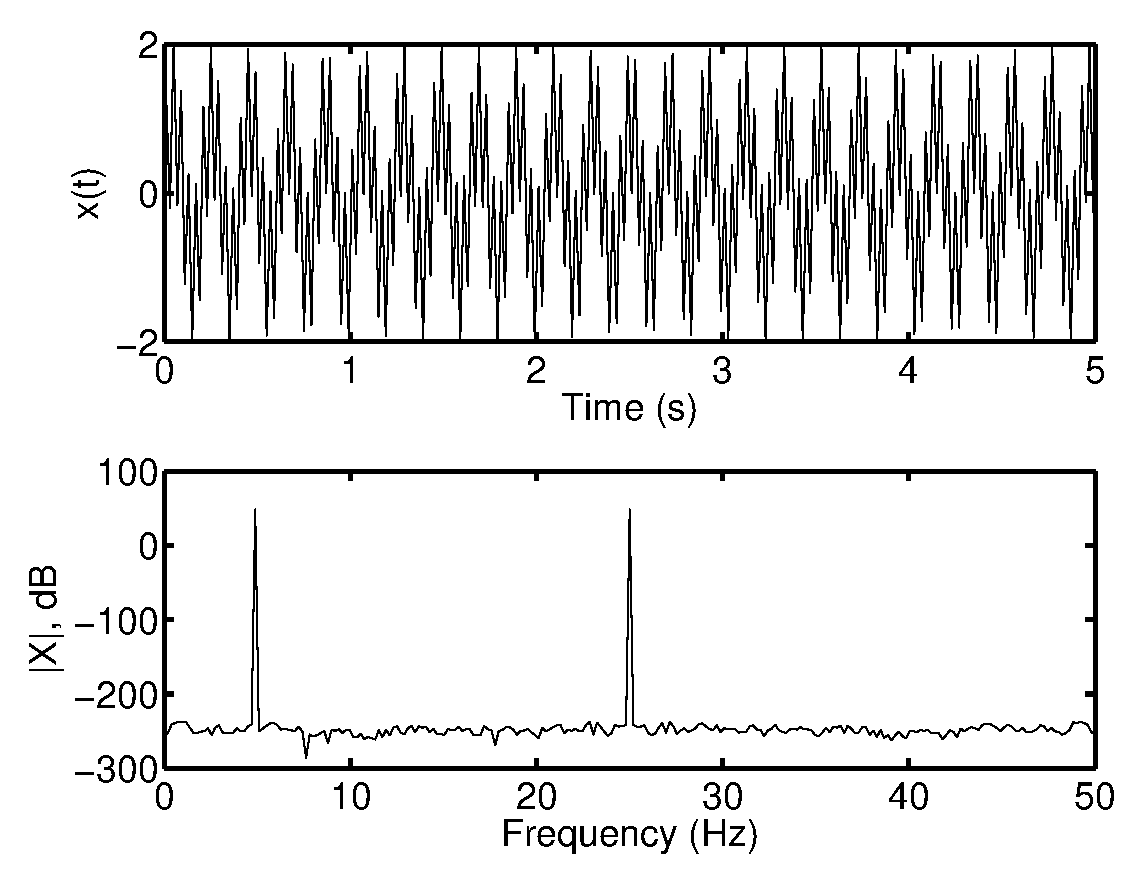
\includegraphics[width=5in]{ch-fft/fft_sin_xX}}
\caption[Sum of two sinusoids with 512 samples and its 
FFT]{Sum of two sinusoids $x$ with $N=512$ samples (top) and its
FFT $|X|$ (bottom). The sampling frequency is $f_s=100$Hz, $f_1=25
\Delta f=4.8828$Hz and $f_2=128 \Delta f=25.0$Hz, where frequency step
$\Delta f=f_s/N=0.1953$Hz/sample.
\label{fig:fft-sin-xX}}
\end{figure}

The corresponding frequency step in Hz is $\Delta f=f_s/N$, so
$\hat{f}=k \Delta f$, $k=0, 1,2,\ldots, N/2$. First, let's use $N=512$
and set the frequency components of the signal to be $f_1=25 \Delta
f=4.8828$Hz and $f_2=128 \Delta f=25.0$Hz. The signal and its FFT
result are shown on the top and bottom of figure~\ref{fig:fft-sin-xX}.
\index{Discrete Fourier Transform (DFT)!of sum of two sinusoids}

As we expected, the two components appear in locations 4.8828Hz and
25.0Hz. Their magnitudes are around 300dB. Theoretically, all other
value should be zero except these two. The nonzero values away from
these two frequencies represent unavoidable computational errors
introduced.

\begin{figure}
\centerline{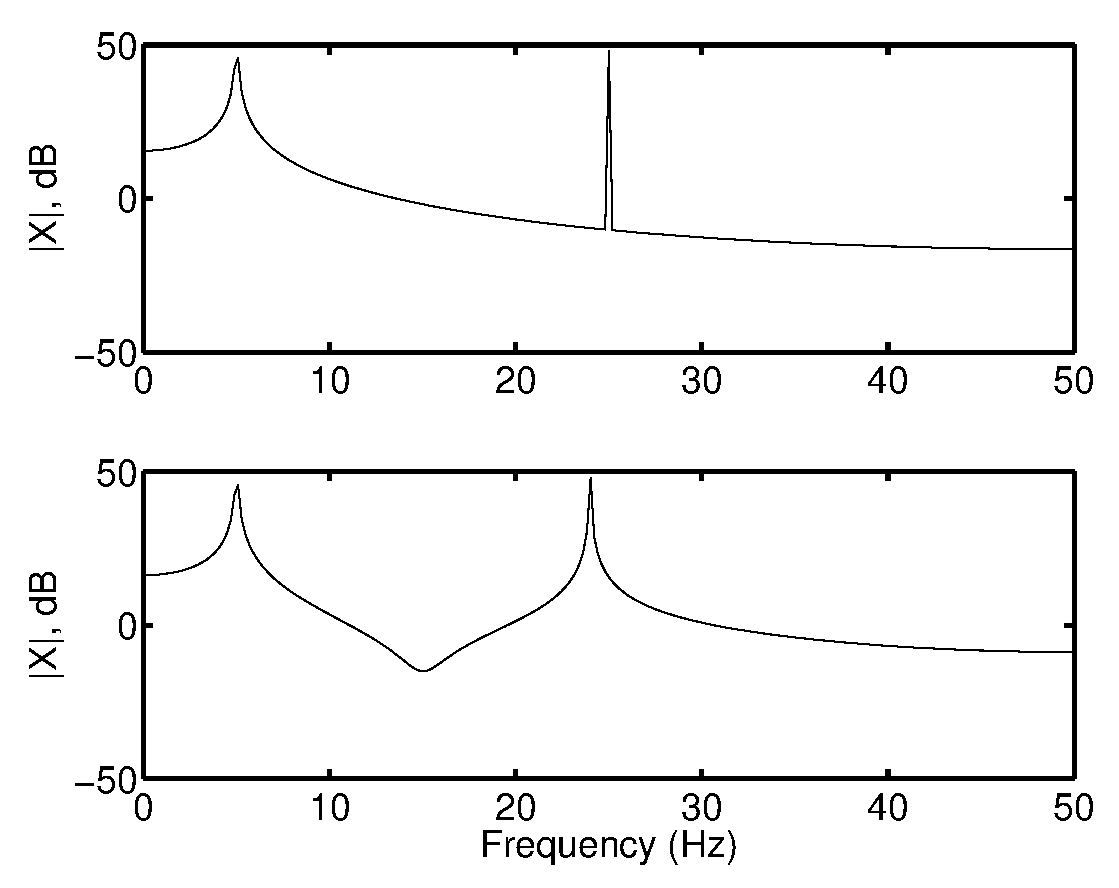
\includegraphics[width=5in]{ch-fft/fft-leakage}}
\caption[Sum of two sinusoids with 512 samples and its  
FFT; different frequencies]{Similar input signals as in
figure~\protect\ref{fig:fft-sin-xX}, but here the two frequencies are
$f_1=5$Hz and $f_2=25$Hz for the top plot and $f_1=5$Hz and $f_2=24$Hz
for the bottom.
\label{fig:fft-leakage}}
\end{figure}

Now, let's choose another a pair of frequency values, $f_1=5$Hz and
$f_2=25$Hz and check the result in figure~\ref{fig:fft-leakage} (top).

How about $f_1=5$Hz and $f_2=24$Hz?, See figure~\ref{fig:fft-leakage}
(bottom). In both cases in this figure, the peaks are below 40dB, down
from 300dB. Why? This is caused by the discrete nature of the
frequency representation and the fact that one or two of the signal's
frequency components are not lined up with the set of discrete
frequencies $\{\hat{f}\}$ --- they fall in between two DFT points. For
the pair $f_1=5$Hz and $f_2=25$Hz, $f_1=5$Hz falls between the points
$k=25$ and $26$ and $f_2=25$Hz is lined up with $k=128$. So, the first
peak is broad and its energy shows up in significant amounts at all of
the DFT frequencies.  The second one is narrow and sharp, but because
of the first peak's energy distribution, its amplitude is low too
(actually, the amplitudes of all the ``in between'' points have been
raised). For the second pair of $f_1=5$Hz and $f_2=24$Hz, neither are
lined up so both of them are broad and low.

\section{Power Leakage [\textsc{Optional}]}

Power leakage is the phenomenon where power at a particular frequency
(called the \emph{center frequency} or \emph{central lobe}) ``leaks''
into neighboring frequencies, which results in the center frequency
peak being reduced, the peak width becoming broader, and nearby
frequencies' (or side lobes') amplitudes increasing. This happens when
the signal abruptly changes, for instance suddenly turning on or
off. Let's see the case of a truncated signal.

\index{FFT!of finite-duration signals|(}
When we compute a signal's spectrum, values of the signal for all time
are required. However, in practice, we observe signals for only finite
durations. Therefore, the spectrum of a signal can only be
approximated from a finite data record. Let's say we have an analog
signal, we sample it at a rate $f_s$, and we limit the duration of the
signal to the time interval $T_0 = NT_s$, where N is the number of
samples and $T_s=1/f_s$ is the sample interval. We denote the original,
infinite-duration discrete signal as $\{x[n]\}$ and duration limited
signal as $\{y[n]\}$. This is equivalent to multiplying $\{x[n]\}$ by a
rectangular window $w[n]$ of length $N$. That is,
\index{FFT!rectangular window and}
\begin{equation}
y[n] = x[n] w[n]
\end{equation}
where 
\begin{equation}
w[n] = \left\{\begin{array}{ll}
                        1 & 0 \le n \le N-1\\
                        0 & otherwise
          \end{array}\right.
\end{equation}
The rectangular window $w[n]$ sharply chopped the original signal to
get the finite signal $y[n]$.

I'll use a sinusoid as an example for the signal $x[n]$,
\begin{equation}
x[n] = \cos \hat{\omega}_0 n
\end{equation}
Using Euler's formula, the signal also can be written as
\begin{equation}
x[n] = \frac{1}{2}\left(e^{j\hat{\omega}_0 n} + e^{-j\hat{\omega}_0 n}\right)
\end{equation}
The windowed version of this signal is 
\begin{equation}
y[n] = \frac{1}{2}\left(e^{j\hat{\omega}_0 n}
       + e^{-j\hat{\omega}_0 n}\right)w[n]
\end{equation}

Setting $\hat{\omega}_k = k2\pi/N$ (the $N$ radian/sample frequency
points in the FFT) in the DFT formula and applying it,
\begin{align}
Y[k] \equiv Y(\hat{\omega}_k) &= \sum_{n=0}^{N-1} w[n]
   \frac{1}{2}(e^{j\hat{\omega}_0 n}
               + e^{-j\hat{\omega}_0 n})e^{-j\hat{\omega}_kn} \notag\\
&= \frac{1}{2}\sum_{n=0}^{N-1} w[n]
   (e^{-j(\hat{\omega}_k-\hat{\omega}_0) n}
    + e^{-j (\hat{\omega}_k+\hat{\omega}_0) n}) \notag\\
&= \frac{1}{2} (W(\hat{\omega}_k-\hat{\omega}_0)
                 + W(\hat{\omega}_k+\hat{\omega}_0))
\label{eq:usefft-Y1}
\end{align}
where $W(\hat{\omega})$ is the DFT of the window $w[n]$. Actually,
$w[n]$ can be viewed as the long pulse we talked about in
chapter~\ref{ch:physical-signals}. Its DFT is
\begin{align}
W[k] \equiv W(\hat{\omega}_k) &= \sum_{n=0}^{N-1} w[n]
    e^{-j\hat{\omega}_k n} \notag\\
&= \sum_{n=0}^{N-1} e^{-j\hat{\omega}_k n}
\label{eq:usefft-rWk1}\\
&= \frac{\sin(\hat{\omega}_k N/2)}{\sin\hat{\omega}_k/2}e^{-j\hat{\omega}_k(N-1)/2}
\label{eq:usefft-rWk2}
\end{align}

\begin{figure}
\centerline{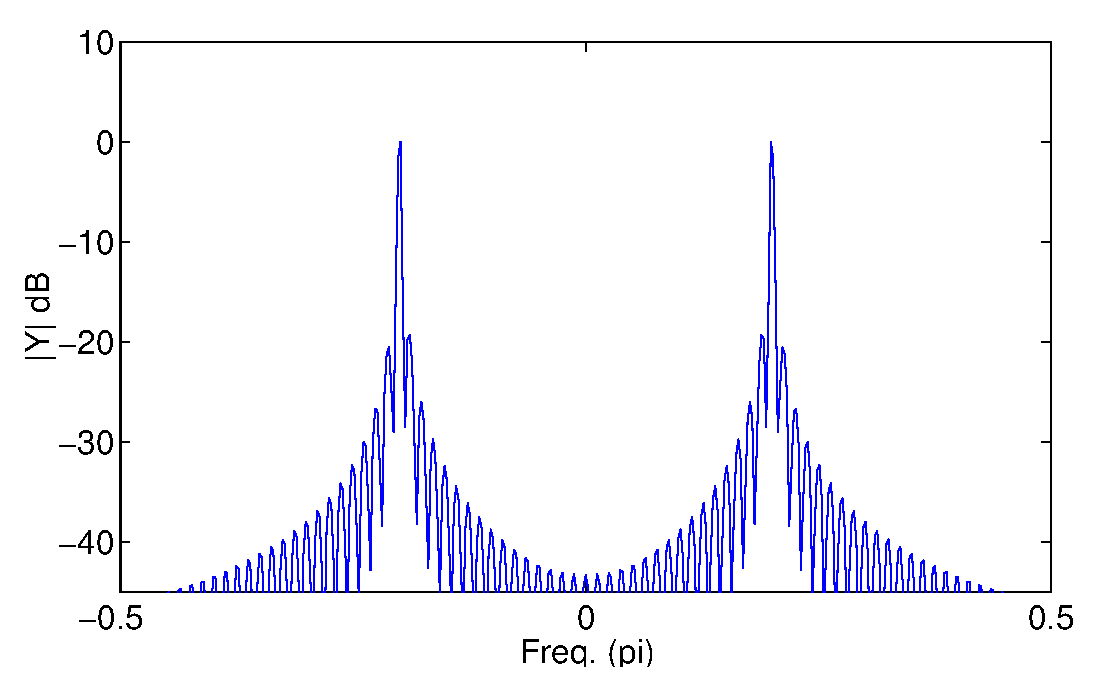
\includegraphics[width=6in]{ch-fft/ufft_cos0-2_rWX}}
\caption[Magnitude spectrum of windowed signal
{$x[n]=\cos\hat{\omega}_0 n$}]{Magnitude spectrum of windowed
signal $x[n]=\cos\hat{\omega}_0 n$, $\hat{\omega}_0=0.2\pi$ and the
rectangular window length is $N=128$. This Illustrates the occurrence
of power leakage.\label{fig:usefft-rWX1}}
\end{figure}

Figure~\ref{fig:usefft-rWX1} is a plot of $Y(\hat{\omega}_k)$ with a
window length of $N=128$, and $\hat{\omega}_0=0.2\pi$. The power of
the original signal sequence $x[n]$ --- concentrated at a single
frequency $\hat{\omega}_0=0.2\pi$ --- has been spread by the
rectangular window into the entire frequency range. That is called
\emph{power leakage}. The rectangular window's effect is to cut out a
piece of the original ``long'' digital signal; this action is
equivalent to turning the signal suddenly on at $n=0$ and off at
$n=N$. This causes the power leakage.
\index{FFT!of finite-duration signals|)}

Let's see what happens if we let the window grow infinity long (or $N
\rightarrow \infty$), that is
\begin{align}
W[n] \equiv W(\hat{\omega}_k)
  &= \sum_{n=0}^{\infty} w[n] e^{-j\hat{\omega}_k n} \notag\\
  &= \sum_{n=0}^{\infty} e^{-j\hat{\omega}_k n}
\end{align}

\begin{figure}
\centerline{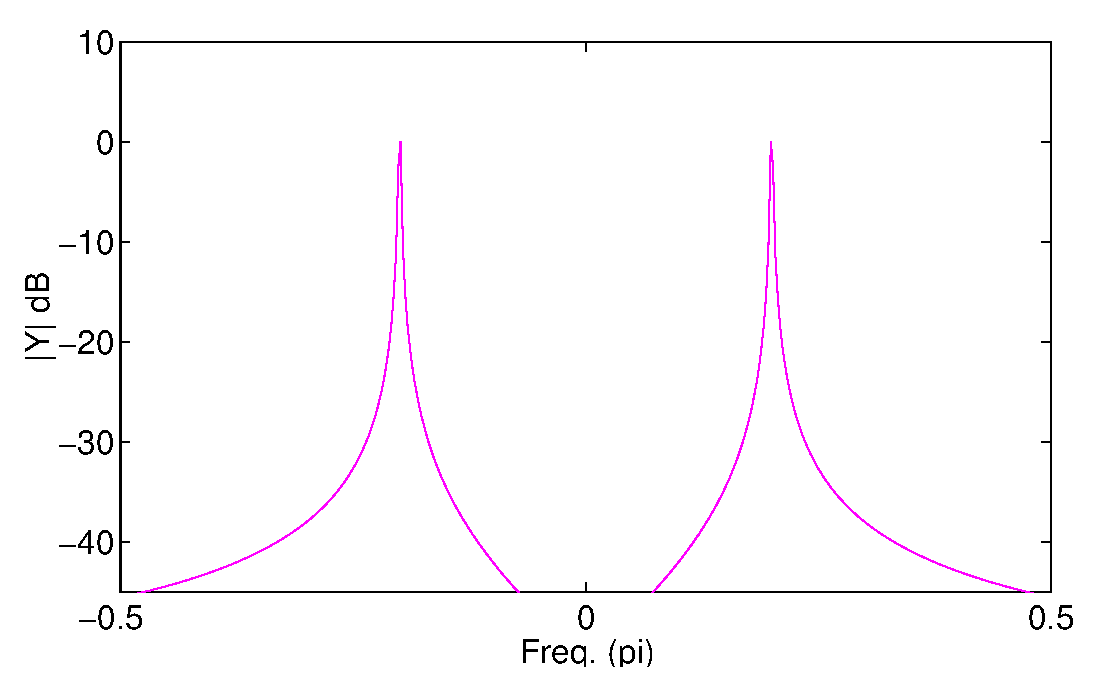
\includegraphics[width=6in]{ch-fft/ufft_cos0-2_rWinfX}}
\caption{Magnitude spectrum of a one-sided signal
$x[n]=\cos\hat{\omega}_0 n$ with
$\hat{\omega}_0=0.2\pi$.\label{fig:usefft-rWinfX}}
\end{figure}

This is an infinite geometric series. Its common ratio is
$e^{-j\hat{\omega}_k}$, so
\begin{align}
W[k] &= \frac{1}{1-e^{-j\hat{\omega}_k}} \notag\\
  &= \frac{1}{2j e^{-j\hat{\omega}_k/2}\sin(\hat{\omega}_k/2)} \notag\\
  &= \frac{-je^{j\hat{\omega}_k/2}}{2\sin(\hat{\omega}_k/2)}
\label{eq:usefft-rWkinf}
\end{align}
Substituting this result back into~(\ref{eq:usefft-Y1}), we obtain the
spectrum of a one-sided signal $x_t$. This is plotted in
figure~\ref{fig:usefft-rWinfX}.

Comparing~(\ref{eq:usefft-rWk2}) and~(\ref{eq:usefft-rWkinf}), the
magnitude of the former has N zeros equally spaced on the frequency
axis, except at the peak frequency $\hat{\omega}_0$, where there is a
$0/0$ situation, which becomes 1. All these zeros contribute to the
spectrum's oscillation. The magnitude of the latter one does not have
a zero.

\problemset{
\subsubsection{Self-Test Exercise}

See~\ref{sc:ch7ex} \#\ref{it:ch7ex1} for the answer.

\begin{enumerate}
\item Fill in the steps leading from~(\ref{eq:usefft-rWk1})
  to~(\ref{eq:usefft-rWk2}).
\end{enumerate}}


\section{Tradeoff Between Time and Frequency Resolution
  [\textsc{Optional}]}

\index{FFT!frequency resolution}
Windowing not only distorts the spectral estimate due to leakage
effects, it also reduces spectral resolution.  There exists a tradeoff
between time and frequency resolution. Wider windows produce finer
frequency resolutions, which means you have the ability to distinguish
between nearby spectral peaks. However, it yields worse time
resolution, meaning that, if you deal with a time-varying signal (a
\index{FFT!of time-varying signals}
signal with spectrum varying along time), the longer the time window is,
the more information is combined within it and the more it
misrepresents \emph{when} the spectral components occurred.

To illustrate the concept of frequency resolution, let's use a digital
signal consisting of three frequency components,
\begin{equation}
x[n] = \cos\hat{\omega}_0 n+\cos\hat{\omega}_1 n + \cos\hat{\omega}_2 n
\label{eq:usefft-cos3a}
\end{equation}
When $x[n]$ is truncated to $N$ samples in the range $0 \le n \le N-1$,
the windowed spectrum is
\begin{equation}
Y(\hat{\omega}_k) =
\frac{1}{2}[W(\hat{\omega}-\hat{\omega}_0)+W(\hat{\omega}-\hat{\omega}_1)
            + W(\hat{\omega}-\hat{\omega}_2)+W(\hat{\omega}+\hat{\omega}_0)
            + W(\hat{\omega}+\hat{\omega}_1)+W(\hat{\omega}+\hat{\omega}_2)]
\label{eq:usefft-cos3}
\end{equation}

\begin{figure}
\centerline{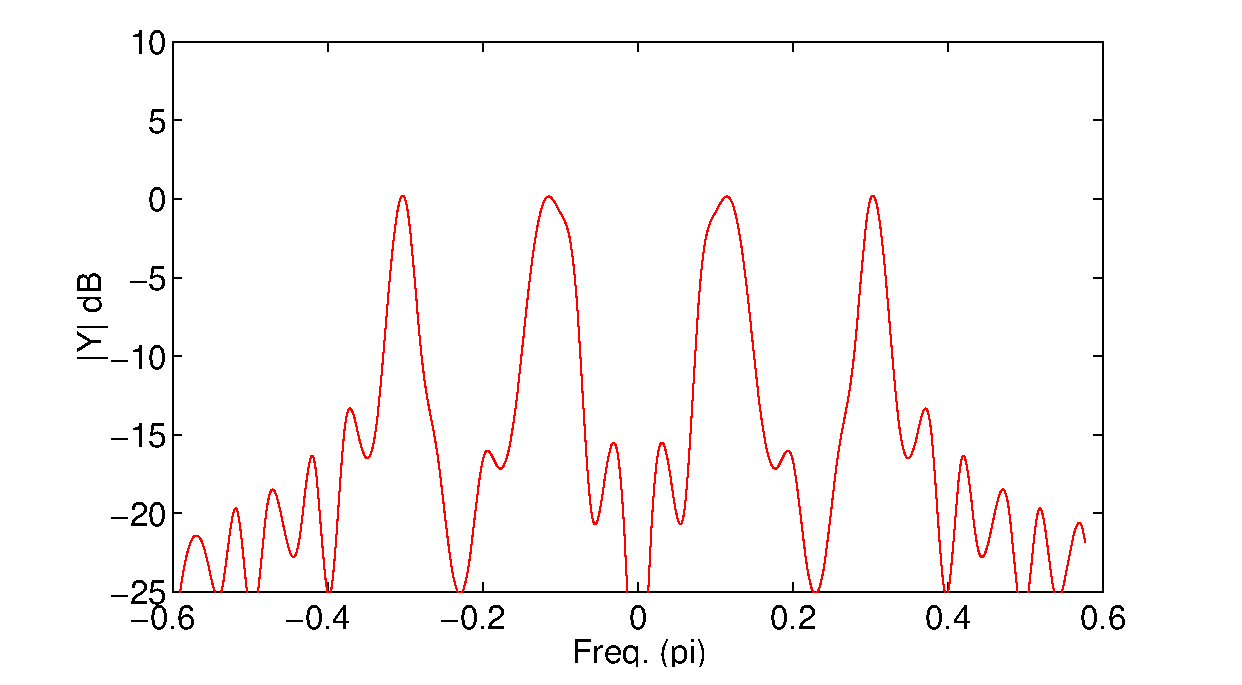
\includegraphics[width=6in]{ch-fft/ufft_cos3_rWX_16}}
\caption[Magnitude spectrum of the 
signal~(\protect\ref{eq:usefft-cos3a}) made up of three
sinusoids]{Magnitude spectrum of the
signal~(\protect\ref{eq:usefft-cos3a}) made up of three sinusoids.
$\hat{\omega}_0=0.1\pi$, $\hat{\omega}_1=0.12\pi$,
$\hat{\omega}_2=0.3\pi$, and the rectangular window length was
$N=16$. Because of the small window size, $\hat{\omega}_0$ and
$\hat{\omega}_1$ are indistinguishable.\label{fig:usefft-rWX3-1}}
\end{figure}

\begin{figure}
\centerline{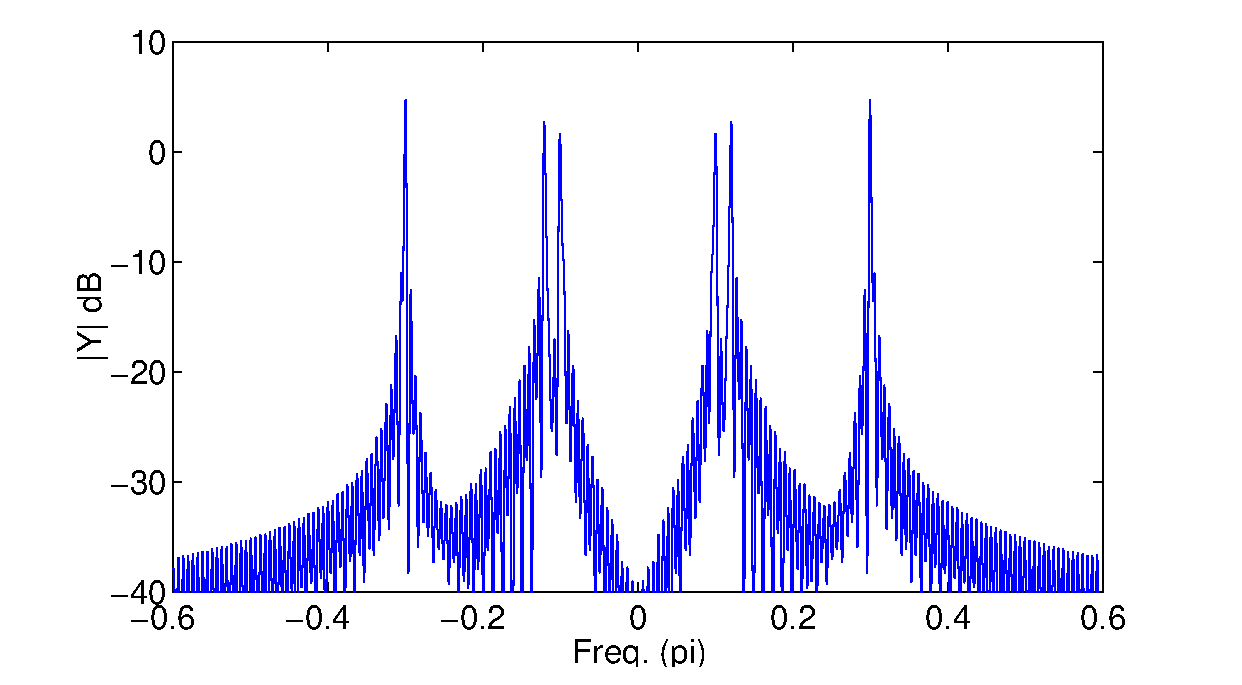
\includegraphics[width=6in]{ch-fft/ufft_cos3_rWX_128}}
\caption[The same figure as~\protect\ref{fig:usefft-rWX3-1}, but with
rectangular window length $N=128$]{The same figure
as~\protect\ref{fig:usefft-rWX3-1}, but the rectangular window length
$N=128$ allows separation of the $\hat{\omega}_0$ and $\hat{\omega}_1$
frequency components.\label{fig:usefft-rWX3-2}}
\end{figure}

Examining~(\ref{eq:usefft-rWk2}) again, the first zero crossing on
either side of the center frequency is the $\hat{\omega}_k$ that
satisfies
\begin{equation}
\frac{\hat{\omega}_k N}{2} = \pi
\end{equation}
which is the first frequency at which $\sin(\hat{\omega}_kN/2)=0$, or
$\hat{\omega}_k=2\pi/N$. The width of the center lobe is twice this,
because there is no zero at $\hat{\omega}_k=0$. The center lobes of
the two window functions $W(\hat{\omega}-\hat{\omega}_i)$ and
$W(\hat{\omega}-\hat{\omega}_j)$ --- corresponding to two frequency
components $\hat{\omega}_i$ and $\hat{\omega}_j$ ($i \ne j$) --- will
overlap if $|\hat{\omega}_i - \hat{\omega}_j|<4\pi/N$.  As a result,
the two spectral lines (peaks) of $x_t$ will be
indistinguishable. Only if $|\hat{\omega}_i - \hat{\omega}_j|\ge
4\pi/N$ can we see two separate lobes in the spectrum
$Y(\hat{\omega}_k)$. Therefore, our ability to resolve spectral lines
of different frequencies is limited by the window main lobe width,
that is $4\pi/N$. As window length $N$ increases, the spacing between
two resolvable frequencies decreases as $1/N$, and so we get better
frequency resolution. Figures~\ref{fig:usefft-rWX3-1}
and~\ref{fig:usefft-rWX3-2} illustrate this conclusion. In these two
figures, the signal has the three components $\hat{\omega}_0=0.1\pi$,
$\hat{\omega}_1=0.12\pi$ and $\hat{\omega}_2=0.3\pi$. The length of
the window for~\ref{fig:usefft-rWX3-1} is $N=16$, where the two close
components $\hat{\omega}_0$ and $\hat{\omega}_1$ are
indistinguishable. The window length for~\ref{fig:usefft-rWX3-2} is
$N=128$, and now we can see two peaks around the $0.1\pi$ area because
the main lobes have become narrow. At the same time, the side lobes
becomes lower, which means that less central frequency power leaks
into neighboring frequencies. This is why the center frequency peak
also becomes higher.

You might then ask if it is always good to extend the window length to
get better frequency resolution. The answer is no. Depending on the
signal, a longer segment might provide worse spectral
information. This is the case when the signal is time-varying, that is
the signal's spectrum changes along time (in every instant, the signal
has different spectrum or frequency components). When we estimate the
spectrum of a windowed signal using the DFT, we treat the segment as
though it were a periodic signal (even though it is not), which
repeats with period equal to the segment length. You can see that, for
a signal that changes with time, this approach mixes together time
domain information from the entire segment. The actual spectrum we get
from a windowed signal is the \emph{average} spectrum in that
window. This means that, for a time-varying signal, a long window will
misrepresent what the actual frequencies are (or, rather it will smear
the frequencies together). The frequency information is all there, but
we don't know \emph{when} they occurred --- we only know that it was
sometime during the window. This suggests that the best approach would
be to decrease the window size to get better time resolution and to
get a more accurate time estimate. Unfortunately, as we just learned,
short windows result in bad frequency resolution. This is the
so-called time/frequency tradeoff. You must do your best to choose a
\index{FFT!time/frequency tradeoff}
window size that meets both your time and frequency resolution
criteria.

A good way to understand this tradeoff is using a \emph{spectrogram},
\index{spectrogram|emph}
or short-time Fourier transform. This is a method to deal with
\index{Fourier transform!short-time|emph}
time-varying signals to get a compromise result for both the time and
frequency domains.  A spectrogram is a sequence of FFT results
produced by a sliding window. Sliding window processing starts at some
time with a fixed window length, computes an FFT, slides the window by
a fixed increment, recomputes the FFT, and repeats this sliding and
FFT computation for the duration of interest. The result is usually
plotted as a surface in a plot with the $X$ axis being time, the $Y$
axis frequency, and surface height being power.  The resulting
spectrogram is a two-dimensional function with independent variables
time and frequency. The magnitude of the spectrogram gives the
spectrum within windows at particular times.

\begin{figure}[p]
\centerline{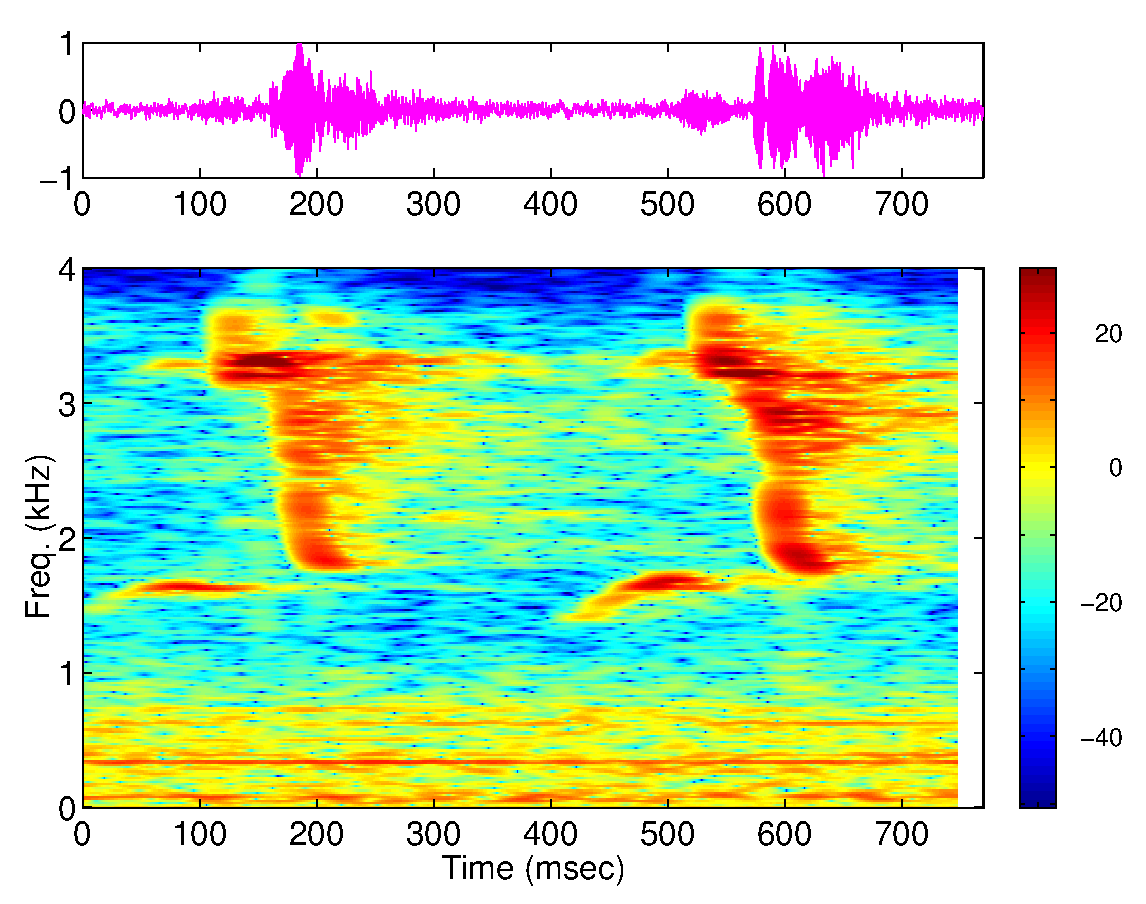
\includegraphics[height=0.35\textheight]{ch-fft/ufft_cardinal1_spg512_511}}
\caption[Bird call waveform and spectrogram; window size 512 samples,
overlap 511]{A bird call waveform (top) and its spectrogram
  (bottom). The window size is 512 samples and the overlap is 511
  samples (increment is 1). Color indicates magnitude, with color key
  on the right of the figure.\label{fig:ufft-birdspg-c1}}
\end{figure}

\begin{figure}
\centerline{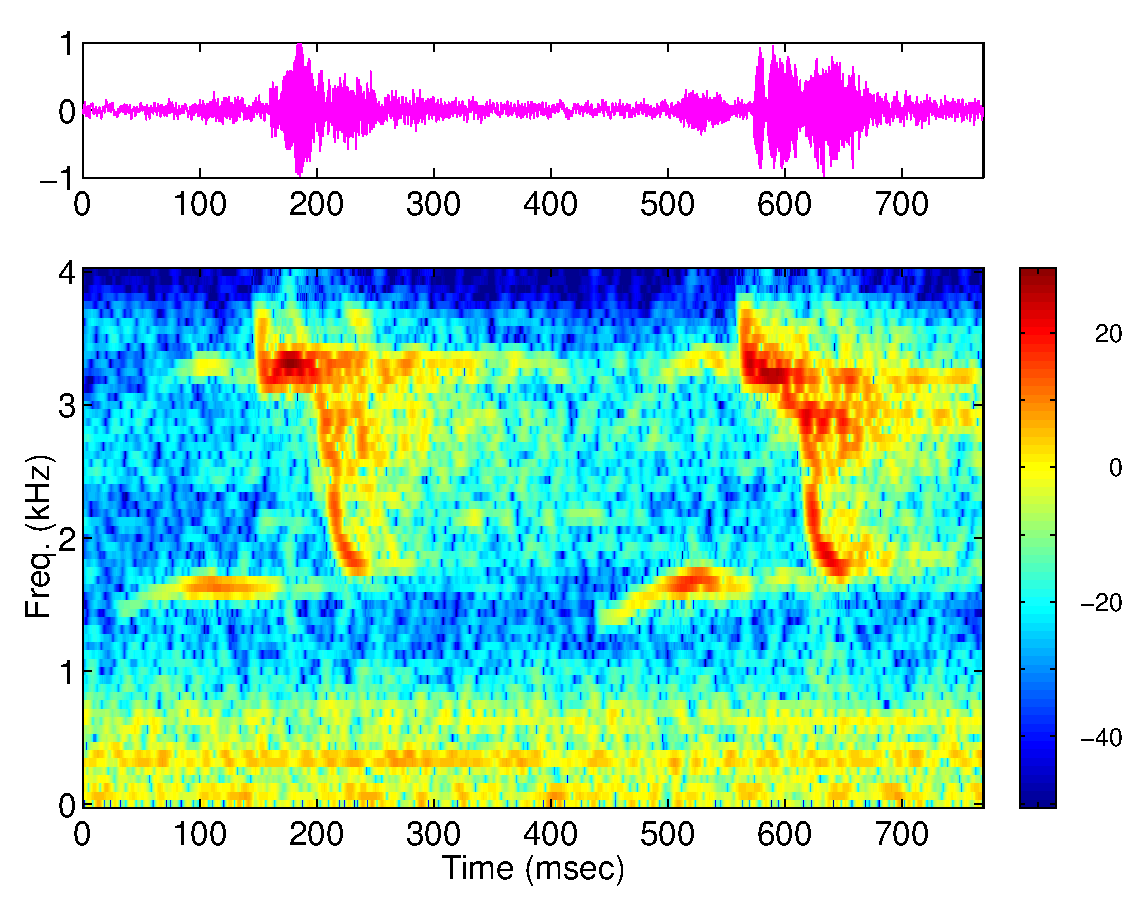
\includegraphics[height=0.35\textheight]{ch-fft/ufft_cardinal1_spg128_127}}
\caption[Bird call waveform and spectrogram; window size 128 samples,
overlap 127]{The same data as figure~\ref{fig:ufft-birdspg-c1}, but
  the window size is 128 samples and overlap is 127 (increment is
  1).\label{fig:ufft-birdspg-c2}}
\end{figure}

\index{spectrogram!of a bird call}
An example of a bird call and its spectrogram is shown in
figures~\ref{fig:ufft-birdspg-c1} and~\ref{fig:ufft-birdspg-c2}. For
each, the top plot is a section of the bird call waveform and the
bottom is a spectrogram with two variables, time and
frequency. Spectrogram color shows the magnitude of the spectrogram
with red high and blue low, as shown by the color bar on the right.

In figure~\ref{fig:ufft-birdspg-c1}, the window length is 512 samples
with an overlap of 511. Let's check the details of the spectral
components with large magnitudes. Starting at the beginning, there is
a component at around 1.5kHz which ends a little before 200
milliseconds. A second component is at around 3.3kHz starting at
approximately 50ms continuing until 300ms, but becoming broader at
around 100ms. Just before this component's end, it has a broad band
frequency range of 1.7kHz to 3.5kHz (time ranging from 150 to
250ms). A similar pattern can be seen in the span of 400--700ms.

Compare this to figure~\ref{fig:ufft-birdspg-c2}, where the window
length is 128 samples. From the point of view of time, the patterns
look narrower, which means they have better temporal resolution
(because of the shorter window). We can now see, for example, that
there is a complex structure in the temporal evolution of the
1.7--3.5kHz frequency band. However, the patterns are broader and
``blockier'' along the frequency axis --- the frequency resolution got
worse (notice the 1.5kHz component in the area of 50--150ms) because
of the short window.

\begin{figure}[p]
\centerline{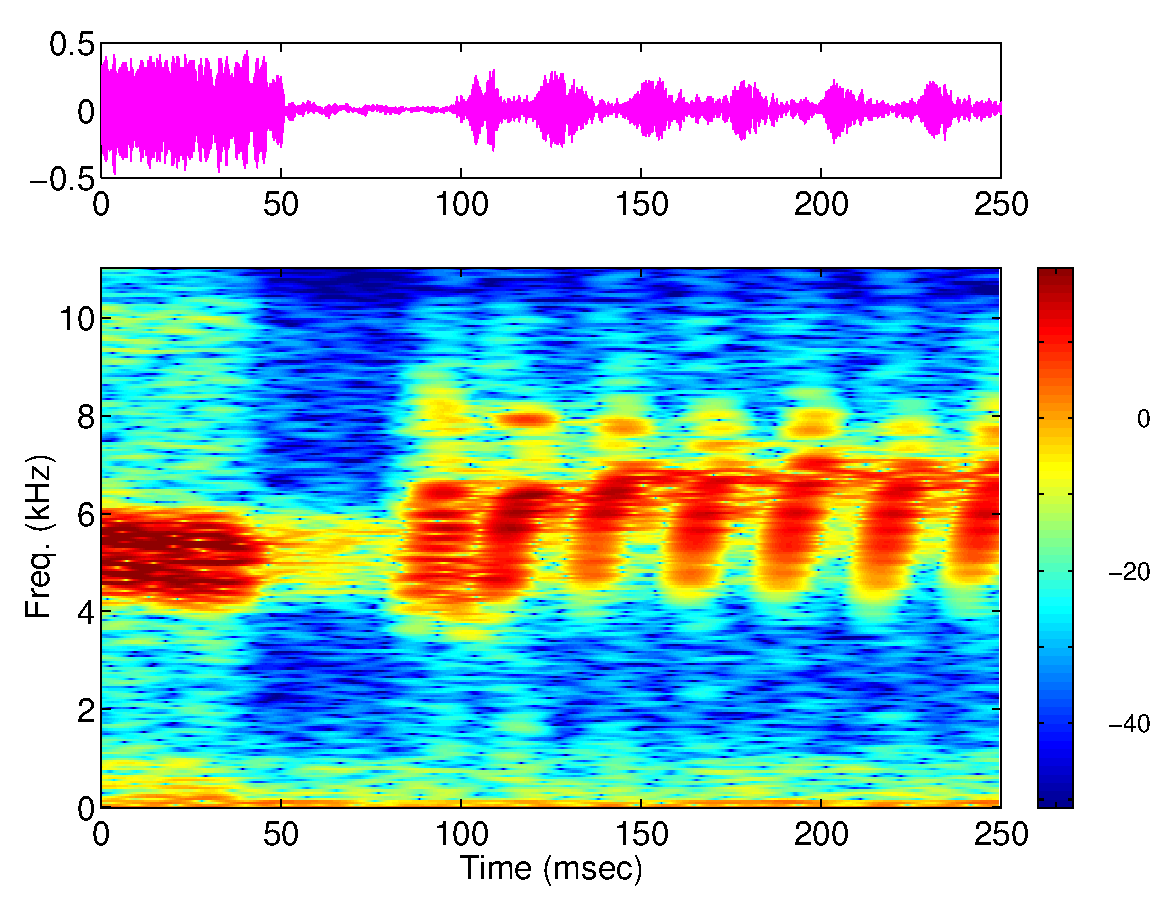
\includegraphics[height=0.4\textheight]{ch-fft/ufft_bluewing1am_spg512_511}}
\caption[Different bird call waveform and spectrogram; 512 sample
window, overlap 511]{Another bird call waveform (top) and its
  spectrogram (bottom), with window size of 512 samples and overlap of
  511 samples.\label{fig:ufft-birdspg-b1}}
\end{figure}

\begin{figure}[p]
\centerline{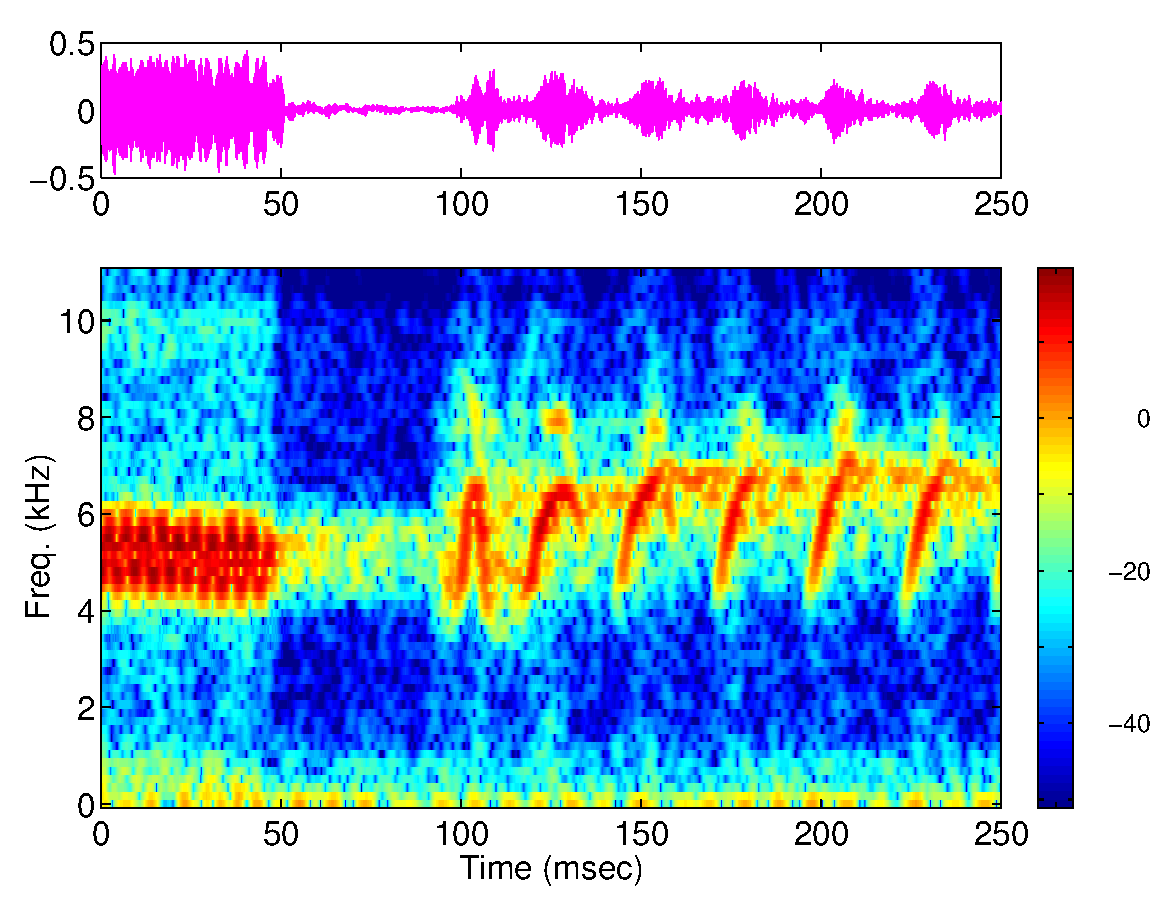
\includegraphics[height=0.4\textheight]{ch-fft/ufft_bluewing1am_spg128_127}}
\caption[Bird call waveform; 128 sample window, overlap 127]{Same data
  as figure~\protect\ref{fig:ufft-birdspg-b1}, but with window size of
  128 samples and overlap of 127.\label{fig:ufft-birdspg-b2}}
\end{figure}

Figures~\ref{fig:ufft-birdspg-b1} and~\ref{fig:ufft-birdspg-b2} are
another pair of examples. They show similar effects from the tradeoff
between time and frequency resolution.

\section{Windowing [\textsc{Optional}]}

The discussion of power leakage has mentioned that turning a signal
on and off suddenly, abruptly truncating it (which is what a
rectangular window does) will cause power leakage from the central
lobe to side lobes. To reduce leakage when we select a segment of a
signal, instead of using an abrupt truncation --- like a rectangular
window produces --- we could select a data window function $w[n]$ that
has lower side lobes in the frequency domain. Examples of some popular
window functions include Hamming, Hann, Bartlett, Blackman, Gaussian,
etc. Each of these has its own characteristics. Some
examples of what these windows look like and what their effects are
presented next.

\subsubsection{Hamming Window}

\begin{figure}
\centerline{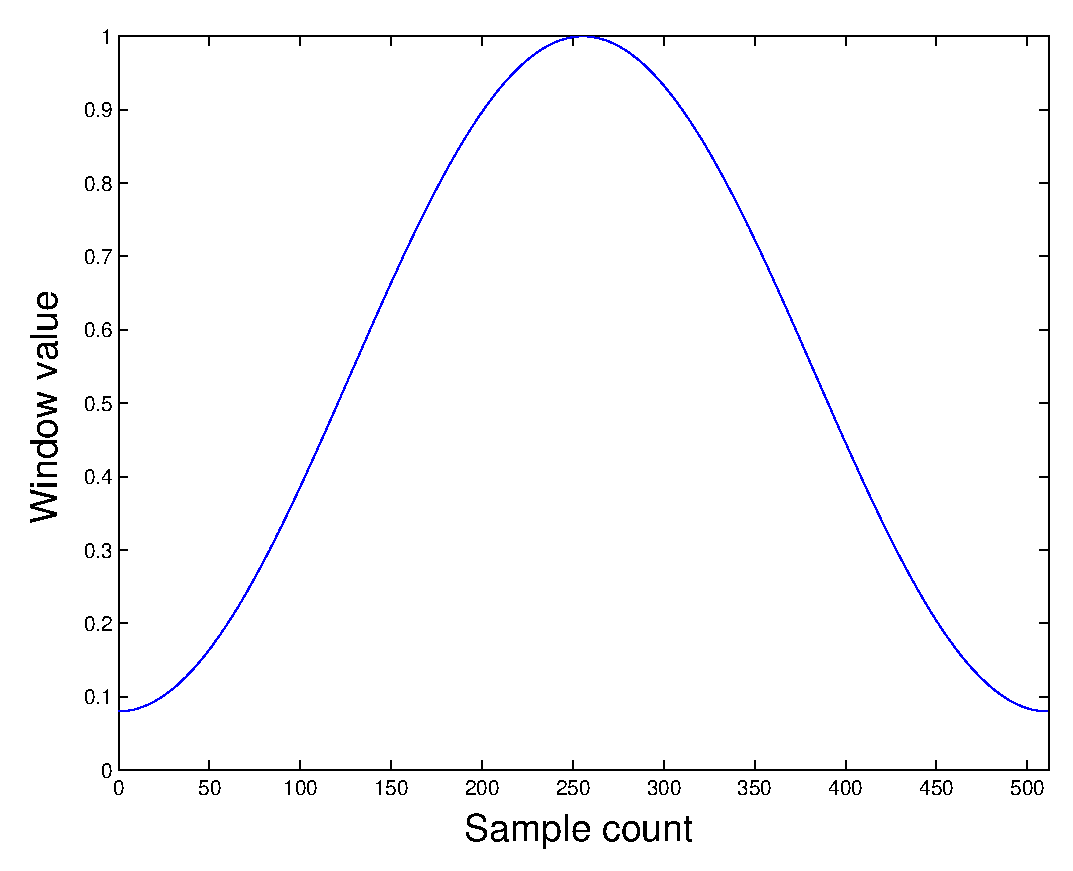
\includegraphics[width=4in]{ch-fft/ufft_hamming_w512}}
\caption{A 512-point Hamming window in the time domain.\label{fig:ufft-hmw}}
\end{figure}

\index{FFT!Hamming window and}
The
coefficients of an $L$-point Hamming window are computed from the
equation,
\begin{equation}
\operatorname{Hamming}[n]
    = 0.54 - 0.46 \cos(2\pi n/(L-1))
          \quad n=0,1,\ldots,L-1
\label{eq:ufft-hnw}
\end{equation}
It consists of a cycle of a cosine, dropping to 0.08 at the end-points
and with a peak value of one. A plot of a Hamming window is shown in
figure~\ref{fig:ufft-hmw}

\subsubsection{Bartlett Window}

\index{FFT!Bartlett window and}
The $L$-point Bartlett window is defined as:

\begin{itemize}
\item For $L$ odd
\begin{equation}
\operatorname{Bartlett}[n]= \left\{\begin{array}{cl}
                        \frac{2n}{L-1}   & 0\le n \le \frac{L-1}{2} \\
                        2-\frac{2n}{L-1} & \frac{L-1}{2}\le n\le L-1
          \end{array}\right.
\end{equation}

\item For $L$ even
\begin{equation}
\operatorname{Bartlett}[n]= \left\{\begin{array}{cl}
                        \frac{2n}{L-1}       & 0\le n \le \frac{L-1}{2} \\
                        \frac{2(L-n-1)}{L-1} & \frac{L-1}{2}\le n\le L-1
          \end{array}\right.
\end{equation}

\end{itemize}

\begin{figure}
\centerline{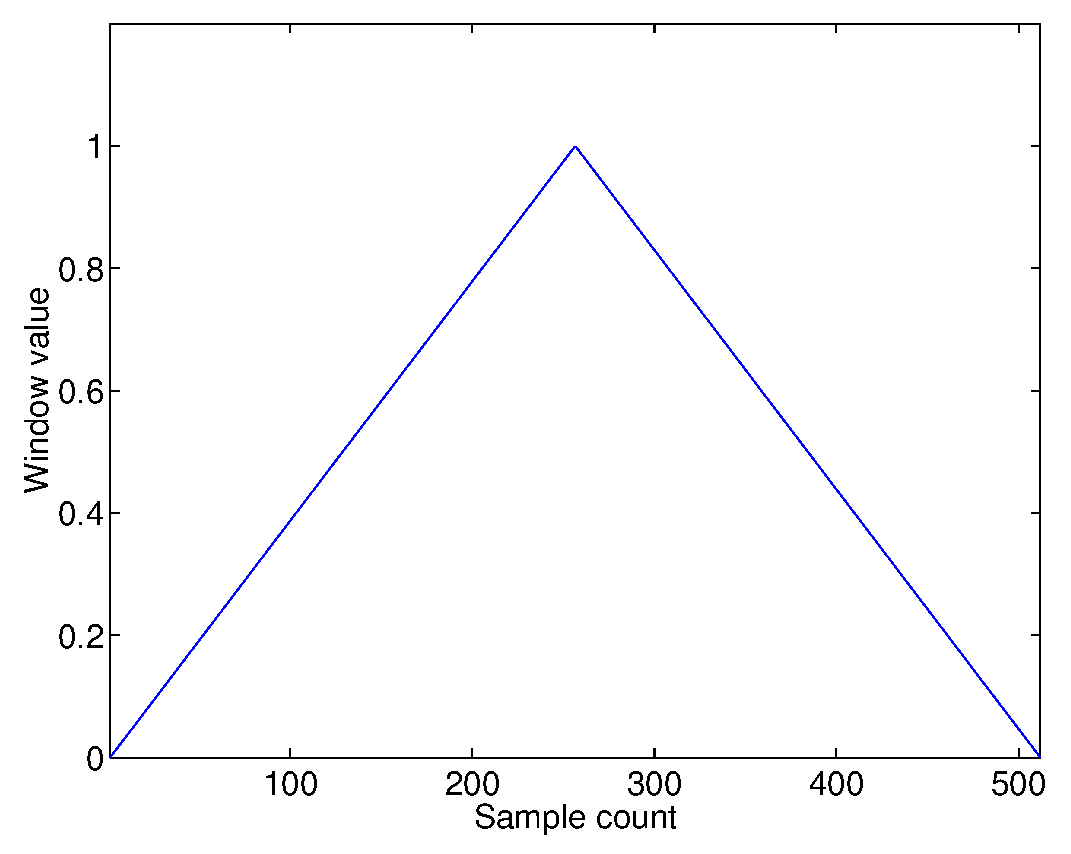
\includegraphics[width=4in]{ch-fft/ufft_bartlett_w512}}
\caption{The 512-point Bartlett window in the time
domain.\label{fig:ufft-baw}}
\end{figure}
 
This is a triangular window with maximum height of one and zeros at
samples 0 and $L-1$. It is plotted in figure~\ref{fig:ufft-baw}.

\subsubsection{Using Window Functions}

How do we use window functions? For a general signal sequence $x[n]$,
the time domain relationship between the windowed sequence $y[n]$ and
original sequence is
\begin{equation}
y[n] = x[n] w[n]
\label{eq:ufft-gw}
\end{equation}
where $w[n]$ is a window function in time domain. The special case of
a rectangular window was previously discussed; now we will consider
$w[n]$ as a general function.

\subsubsection{Example: Windowed Sinusoid}

\begin{figure}
\centerline{\includegraphics[height=0.35\textheight]{ch-fft/ufft_hannrect_cosx512_256}}
\caption[Hann windowed cosine waveform and its spectrum]{Hann windowed
cosine waveform ($\hat{\omega}_0=0.2\pi$) and its spectrum, compared to
rectangular window. The top is the cosine waveform windowed by
rectangular (yellow) and Hann (red) windows, the bottom is their
corresponding spectra.\label{fig:ufft-hnrt-cosx}}
\end{figure}

Consider again a sinusoid signal $x[n]$, 
\begin{equation}
x[n] = \cos(\hat{\omega}_0 n);
\end{equation}
Instead of using a rectangular window, let's first use a Hann window
and see the results. The windowed signal $y[n]$ is
\begin{equation}
y[n] = x[n] \operatorname{Hann}[n]
     = \cos(\hat{\omega}_0 n)\operatorname{Hann}[n]
\end{equation}
where the Hann window is as described in~(\ref{eq:ufft-hnw}). $y[n]$
is shown in figure~\ref{fig:ufft-hnrt-cosx} (top, red curve); its
spectrum is the red curve in the bottom plot. Since $x[n]$ only has
one component $\hat{\omega}_0=0.2\pi$, ideally there should be only
one $\delta$ function peak at frequency $0.2\pi$. However, as you now
know, that is not likely to be the case because of power leakage. The
magnitude value is gradually damped down away from the center lobe
around $\hat{\omega}_0$. The leakage is smaller with the Hann window
than a rectangular one (yellow curves). On the other hand, the
rectangular windowed signal has a narrower peak than the Hann windowed
one. So, we can see that the Hann window decreases power leakage by
sacrificing peak resolution.

\begin{figure}
\centerline{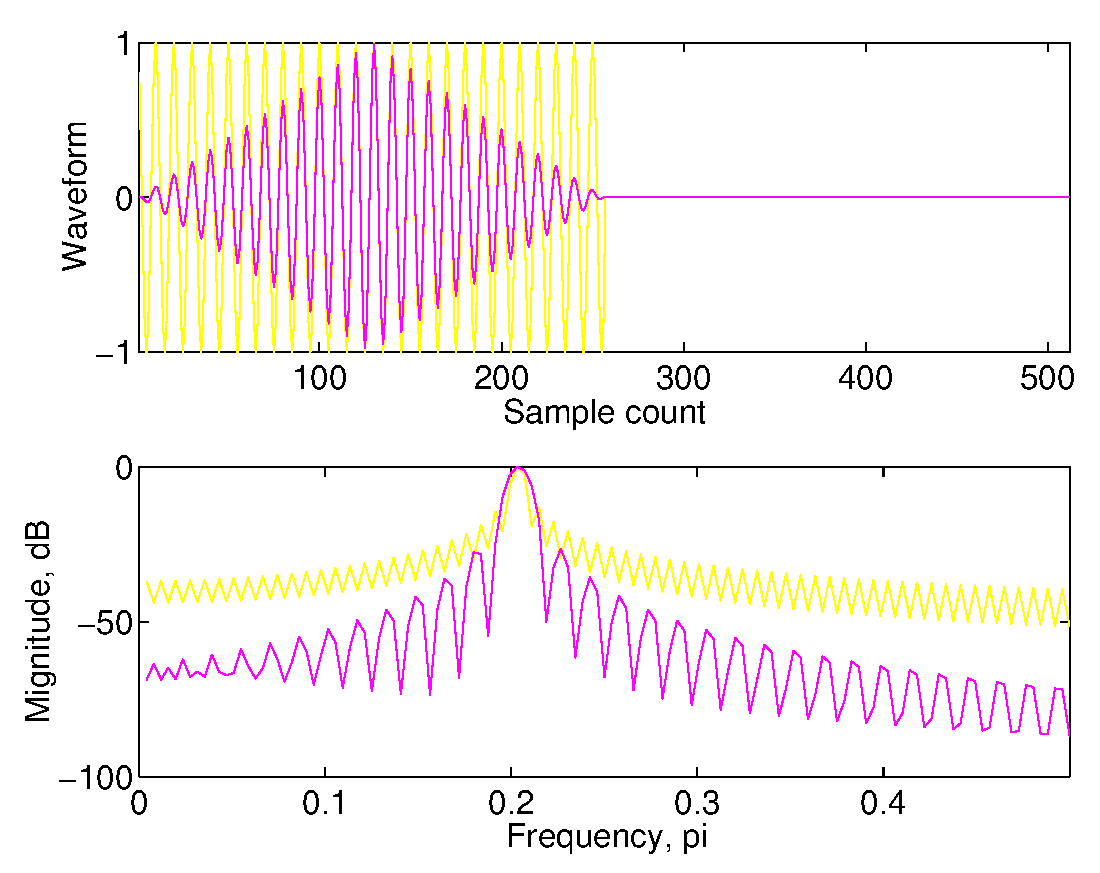
\includegraphics[height=0.35\textheight]{ch-fft/ufft_bartlrect_cosx512_256}}
\caption[Bartlett windowed cosine waveform and its spectrum]{Bartlett
windowed cosine waveform and its spectrum, compared to rectangular
window. The top is the cosine waveform windowed by rectangular
(yellow) and Bartlett (magenta), the bottom is their corresponding
spectra.\label{fig:ufft-bart-cosx}}
\end{figure}

Let's see the result of using a Bartlett window. For the same cosine
waveform, the results are shown in figure~\ref{fig:ufft-bart-cosx}.
We can reach similar conclusions about the Bartlett window. But, there
is a difference between the two windows, as you can see in
figure~\ref{fig:ufft-hnba-cosx}, which is a comparison between the
Hann and Bartlett windows for the cosine wave. Though it appears that
the Hann window is superior, there are a number of issues (beyond the
scope of this book) that we won't discuss; the choice of window
function involves a number of tradeoffs and depends on the signals
being processed and the goal of the processing.

\begin{figure}
\centerline{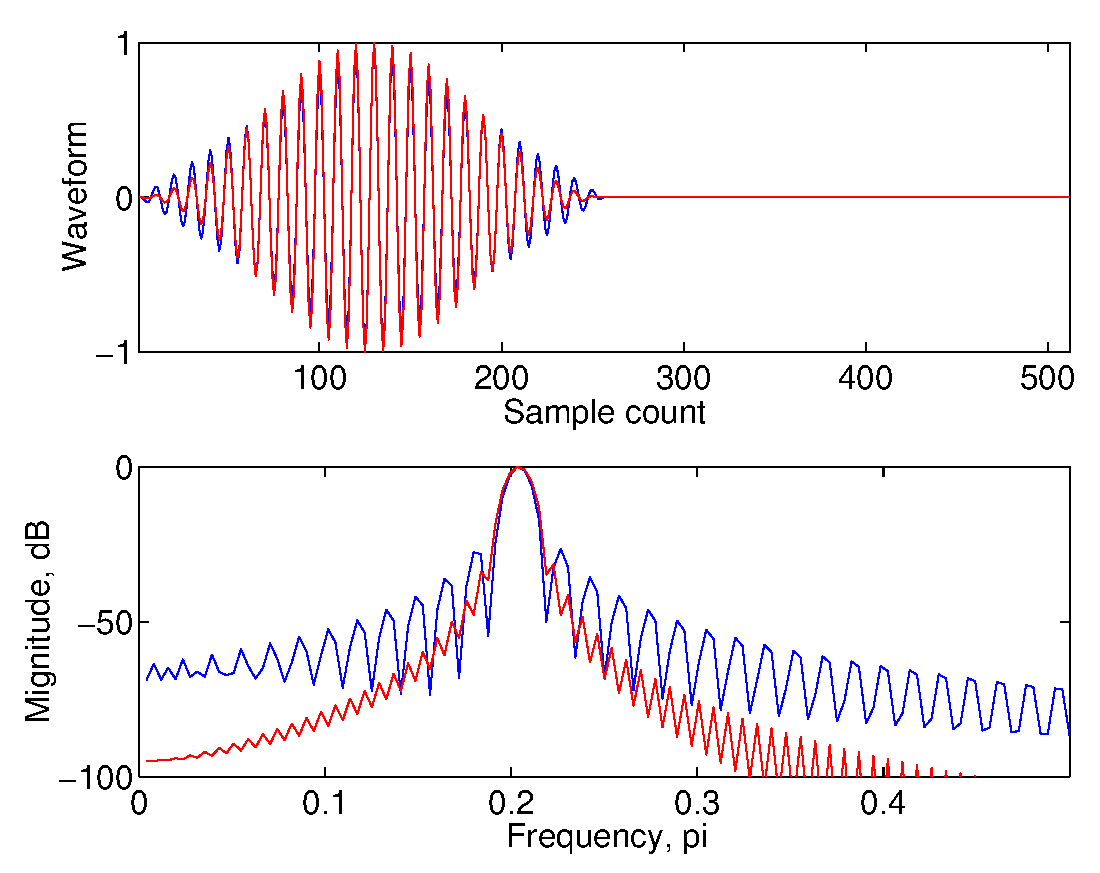
\includegraphics[height=0.35\textheight]{ch-fft/ufft_hannbartl_cosx512_256}}
\caption[Comparison between Hann and Bartlett windows for
a cosine wave]{Comparison between Hann (red, lower curve) and Bartlett
(blue, upper curve) windows for a cosine
wave.\label{fig:ufft-hnba-cosx}}
\end{figure}

\subsubsection{Example: Windowed Bird Call}

\begin{figure}
\centerline{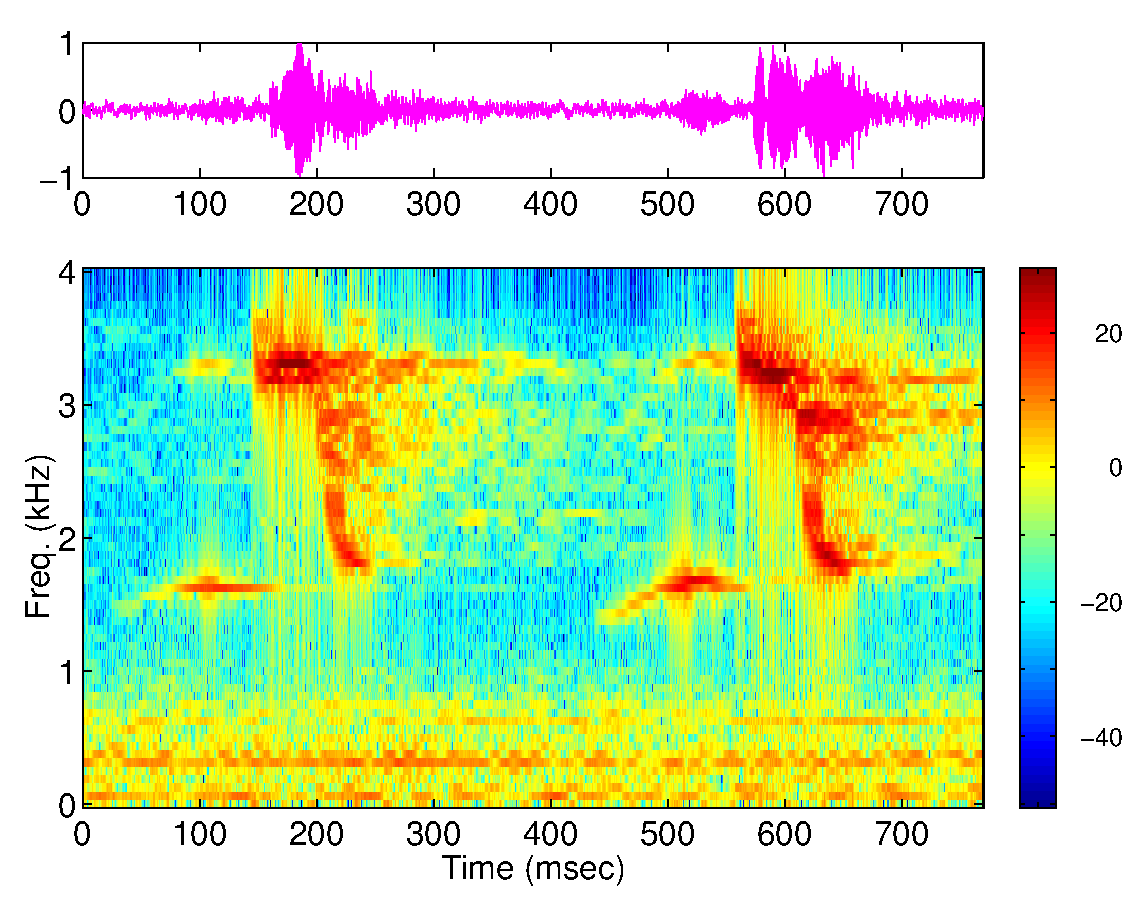
\includegraphics[height=0.35\textheight]{ch-fft/ufft_cardinal1_spg128_127rect}}
\caption{Similar spectrogram as
figure~\protect\ref{fig:ufft-birdspg-c2}, but here a rectangular
window is used.\label{fig:ufft-birdspg-c3}}
\end{figure}

\index{spectrogram!of a bird call}
Here, let's once again examine the bird call spectrogram I introduced
earlier. When that spectrogram was presented, a cheat was used: a Hann
window, instead of a rectangular one. Now, instead of using a Hann
window in figure~\ref{fig:ufft-birdspg-c2}, if a rectangular one is used,
we get figure~\ref{fig:ufft-birdspg-c3}. The increased power leakage
into the side lobes of the two main frequency components is readily
apparent. This leakage messes up the spectral appearance and affects
how accurately we can estimate the shape of the frequency components.
That illustrates how important it is to choose the right window.

\begin{figure}
\centerline{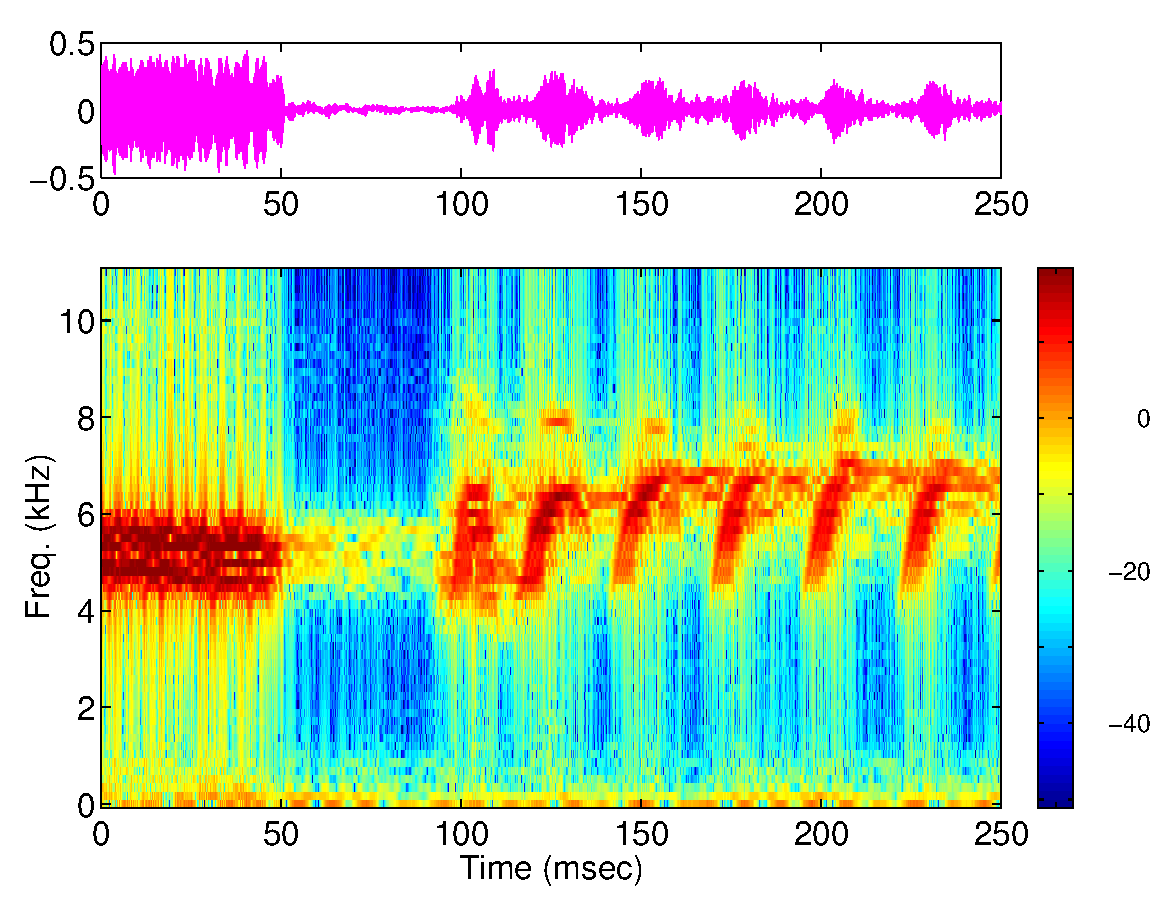
\includegraphics[height=0.5\textheight]{ch-fft/ufft_bluewing1am_spg128_127rect}}
\caption{Similar spectrogram as figure~\ref{fig:ufft-birdspg-b2}, but
here a rectangular window is used.\label{fig:ufft-birdspg-b3}}
\end{figure}

Figure~\ref{fig:ufft-birdspg-b3} presents a similar result for the
bird call originally Hann windowed in
figure~\ref{fig:ufft-birdspg-b2}.

\problemset{
\subsubsection{Self-Test Exercise}

See~\ref{sc:ch7ex} \#\ref{it:ch7ex2} for the answer.

\begin{enumerate}
\item Plot the Hann and Hamming windows in the time domain and compare
their shapes.
\end{enumerate}}

\section{Problems}

\begin{enumerate}
\item If $x(t)=100\sin 20\pi t$ for $-0.05<t<0.05$ and $x(t)=0$ for
$t<-0.05$ and $t>0.05$, evaluate its Fourier transform at $\omega=$
(a) 0, (b) $10\pi$, (c) $-10\pi$, (d) $20\pi$.

\item Trace by hand the 8-point FFT algorithm for the following signals,
  showing the intermediate steps. Plot their magnitude spectra.
\begin{enumerate}
\item $x[n] = \{-1, 1, -1, 1, -1, 1, -1, 1\} $

\item $x[n] = \{0,1,1,0,1,1,0,1\}$

\item $x[n] = \{0,1,2,0,1,2,0,1\}$

\item $x[n] = \{0,1,2,3,0,1,2,3\}$
\end{enumerate}

\item Use your favorite programming language to implement the
iterative FFT defined in algorithm~\ref{alg:fft}.

\item Use Matlab's built-in FFT subroutine to compute the following
DFTs and plot the magnitudes $|X_k|$ of those DFTs using Matlab.
\begin{enumerate}
\item The 64-point DFT of the sequence
\begin{equation*}
x[n]=\left\{\begin{array}{ll}
                        1 &  n=0,1,\ldots,15 \\
                        0 &  \text{otherwise}
           \end{array}\right.
\end{equation*}

\item The 64-point DFT of the sequence 
\label{it:64}
\begin{equation*}
x[n]=\left\{\begin{array}{ll}
                        1 & n=0,1,\ldots,7 \\
                        0 & \text{otherwise}
           \end{array}\right.
\end{equation*}

\item The 128-point DFT of the sequence in~\ref{it:64}.

\item The 64-point DFT of the sequence 
\begin{equation*}
x[n]=\left\{\begin{array}{ll}
                        10e^{n\pi/8}  & n=0,1,\ldots,64 \\
                        0             & \text{otherwise}
           \end{array}\right.
\end{equation*}
\end{enumerate}

Answer the following questions:
\begin{enumerate}\setcounter{enumii}{4}
\item What is the frequency interval between successive samples for the
plots in (a--d)?

\item What is the value of the spectrum at zero frequency (DC value)
in the plots in (a--d)?
\end{enumerate}

\item It is common practice to \emph{normalize} windows by assuring
that the sum of their values is equal to one, i.e.,
\[ \sum_{n=0}^{L-1} w[n] = 1 \]. Show that the Hamming window is
normalized by dividing its values by $0.54L-0.46$.
\item Given the bird call data at
\htmladdnormallink{http://courses.washington.edu/css457/ebook/amoriole2-1.txt}{http://courses.washington.edu/css457/ebook/amoriole2-1.txt}
(4000 samples), and its sampling frequency $f_s=8$kHz, use MATLAB to
compute its spectrogram, plot the waveform and its spectrogram (use
window sizes of 128 and 512 with Hann [hanning] windows and an
increment of 1). Use only the base MATLAB toolbox (\emph{not} the
Signal Processing Toolbox). Submit the resulting figures and code.
\end{enumerate}

\section{Further Reading}

\begin{itemize}
\item James H McClellan, Ronald W. Schafer, and Mark A. Yoder,
  \textit{DSP First: A Multimedia Approach}, Prentice Hall, 1998,
  chapter 9.
\end{itemize}


% LocalWords:  spectrum's Hann MATLAB
